% !TeX root = NCM-TFG.tex
%%***********************************************
%% Plantilla para TFG.
%% Escuela Técnica Superior de Ingenieros Informáticos. UPM.
%%***********************************************
\documentclass[a4paper,11pt]{book}
% -*-coding: utf-8 -*-
%%***********************************************
%% Plantilla para TFG.
%% Escuela Técnica Superior de Ingenieros Informáticos. UPM.
%%***********************************************
%% Preámbulo del documento.
%%***********************************************
\usepackage[utf8]{inputenc}
\usepackage[T1]{fontenc}
\usepackage[english,spanish,es-lcroman]{babel}
\usepackage{bookman}
\decimalpoint
\usepackage{graphicx}
\usepackage{amsfonts,amsgen,amsmath,amssymb}
\usepackage[top=3cm, bottom=3cm, right=2.54cm, left=2.54cm]{geometry}
\usepackage{afterpage}
\usepackage{colortbl,longtable}
\usepackage[pdfborder={0 0 0}]{hyperref}
\usepackage{pdfpages}
\usepackage {tabulary}
\usepackage {array}
\usepackage {xltabular}
\usepackage{booktabs}
\usepackage{float}
\usepackage{tocloft}
\usepackage{tikz}
\usepackage{nameref}
\usepackage{url}
\usepackage{enumitem} % para listas 
\usepackage[stable]{footmisc}
\usepackage{parskip} % para separar párrafos con espacio
\usepackage{svg}
\usepackage[outputdir=build,cache=false]{minted}
\usemintedstyle{vs}
\setminted[typescript]{%
   breaklines,
   mathescape,
   linenos,
   numbersep=5pt,
   frame=single,
   numbersep=5pt,
   xleftmargin=0pt
}
\setminted[bash]{%
   breaklines,
   mathescape,
   linenos,
   numbersep=5pt,
   frame=single,
   numbersep=5pt,
   xleftmargin=0pt
}
\setminted[json]{%
   breaklines,
   mathescape,
   numbersep=5pt,
   frame=single,
   numbersep=5pt,
   xleftmargin=0pt,
   breakanywhere
}

\usepackage{titlesec}
\titlespacing{\section}{0pt}{\parskip}{0pt}
\titlespacing{\subsection}{0pt}{\parskip}{0pt}
\setlength{\intextsep}{5pt}

%%-----------------------------------------------
\usepackage{fancyhdr}
\pagestyle{fancy}
\fancyhf{}
\fancyhead[LO]{\leftmark}
\fancyhead[RE]{\rightmark}
\setlength{\headheight}{1.5\headheight}
\cfoot{\thepage}

\addto\captionsspanish{ \renewcommand{\contentsname}
   {Tabla de contenidos} }
\setcounter{tocdepth}{4}
\setcounter{secnumdepth}{4}

\renewcommand{\chaptermark}[1]{\markboth{\textbf{#1}}{}}
\renewcommand{\sectionmark}[1]{\markright{\textbf{\thesection. #1}}}
\newcommand{\HRule}{\rule{\linewidth}{0.5mm}}
\newcommand{\bigrule}{\titlerule[0.5mm]}

\usepackage{appendix}
\renewcommand{\appendixname}{Anexos}
\renewcommand{\appendixtocname}{Anexos}
%\renewcommand{\appendixpagename}{Anexos}
%%-----------------------------------------------
%% Páginas en blanco sin cabecera:
%%-----------------------------------------------
\usepackage{dcolumn}
\newcolumntype{.}{D{.}{\esperiod}{-1}}
\makeatletter
\addto\shorthandsspanish{\let\esperiod\es@period@code}

\def\clearpage{
   \ifvmode
      \ifnum \@dbltopnum =\m@ne
         \ifdim \pagetotal <\topskip
            \hbox{}
         \fi
      \fi
   \fi
   \newpage
   \thispagestyle{empty}
   \write\m@ne{}
   \vbox{}
   \penalty -\@Mi
}
\makeatother
%%-----------------------------------------------
%% Estilos código de lenguajes: Consola, C, C++ y Python
%%-----------------------------------------------
\usepackage{color}

\definecolor{gray97}{gray}{.97}
\definecolor{gray75}{gray}{.75}
\definecolor{gray45}{gray}{.45}

\usepackage{listings}
\lstset{ frame=Ltb,
   framerule=0pt,
   aboveskip=0.5cm,
   framextopmargin=3pt,
   framexbottommargin=3pt,
   framexleftmargin=0.4cm,
   framesep=0pt,
   rulesep=.4pt,
   backgroundcolor=\color{gray97},
   rulesepcolor=\color{black},
   %
   stringstyle=\ttfamily,
   showstringspaces = false,
   basicstyle=\scriptsize\ttfamily,
   commentstyle=\color{gray45},
   keywordstyle=\bfseries,
   %
   numbers=left,
   numbersep=6pt,
   numberstyle=\tiny,
   numberfirstline = false,
   breaklines=true,
}
\lstnewenvironment{newlisting}[1][]
{\lstset{#1}\pagebreak[0]}{\pagebreak[0]}

\lstdefinestyle{consola}
{basicstyle=\scriptsize\bf\ttfamily,
   backgroundcolor=\color{gray75},
}

\lstdefinestyle{CodigoC}
{basicstyle=\scriptsize,
   frame=single,
   language=C,
   numbers=left
}

\lstdefinestyle{CodigoC++}
{basicstyle=\small,
   frame=single,
   backgroundcolor=\color{gray75},
   language=C++,
   numbers=left
}

\lstdefinestyle{Python}
{language=Python,
}
\makeatother
%%-----------------------------------------------
%% Cargar datos relativos al TFG:
%% (actualizar estos datos en secciones/_DatosTFG.tex) 
%%***********************************************
%% Plantilla para TFG.
%% Escuela Técnica Superior de Ingenieros Informáticos. UPM.
%%***********************************************
%% Información requerida para completar la portada.
%%*********************************************** 

%% Escribe Nombre y Apellidos del autor del trabajo:
\newcommand{\NombreAutor}{ Nicolás Cossío Miravalles }

%% Escribe el Grado: 
\newcommand{\Grado}{ Grado en Ingeniería Informática }

%% Escribe el Título del Trabajo:
\newcommand{\TituloTFG}{ Desarrollo de un Sistema de Intercambio Directo de Archivos entre Dispositivos Basado en IPFS} 

%% Escribe Nombre y Apellidos del Tutor del trabajo: 
\newcommand{\NombreTutor}{ Fernando Pérez Costoya } 

% Escribe el Departamento al que pertenece el Tutor:
\newcommand{\Departamento}{ Arquitectura Y Tecnología De Sistemas Informáticos }

% Escribe la fecha de lectura, en formato: Mes - Año
\newcommand{\Fecha}{ Abril - 2023 }
%%***********************************************

\listfiles

%%-----------------------------------------------
%% Documento:
\begin{document}
%%***********************************************
%% Plantilla para TFG.
%% Escuela Técnica Superior de Ingenieros Informáticos. UPM.
%%***********************************************
%% Portada. 
%%***********************************************
\begin{titlepage}

  \begin{minipage}{0.15\linewidth}
    \hspace*{-2.5cm}
    \noindent
    
\includegraphics[scale=0.5]{./include/EscUpm.png} \qquad\qquad
  \end{minipage}
  \begin{minipage}{0.7\linewidth}
    \begin{center}
      \huge{ Universidad Politécnica\\de Madrid }\\
      \vspace*{0.5cm}
      \Large{\textbf{Escuela Técnica Superior de \\
          Ingenieros Informáticos}}
    \end{center}
  \end{minipage}
  \begin{minipage}{0.2\linewidth}
    
\includegraphics[scale=0.5]{./include/FacInformatica.png}
  \end{minipage}

  \vspace*{1cm}
  \begin{center}
    \Large{Grado en  \Grado{} }
  \end{center}

  \vspace*{1cm}
  \begin{center}
    \huge{ Trabajo Fin de Grado }
  \end{center}

  \vspace*{0.5cm}
  \begin{center}
    \huge\bfseries {  \TituloTFG{} }
  \end{center}

  \vspace*{5cm}

  \noindent
  \large{Autor: \NombreAutor{} }\\
  \large{Tutor(a): \NombreTutor{} }


  \vspace*{4cm}
  \begin{center}
    Madrid, \Fecha
  \end{center}

  %%--------------------------------
  \newpage
  \thispagestyle{empty}
  %%--------------------------------
  \noindent
  Este Trabajo Fin de Grado se ha depositado en la ETSI Informáticos de la Universidad Politécnica de Madrid para su defensa.

  \vspace*{4cm}
  \noindent
  \textit{Trabajo Fin de Grado}\\
  \textit{Grado en} \Grado{}

  \begin{enumerate}
    \item[\textit{Título:}] \TituloTFG{}
  \end{enumerate}
  \Fecha


  \vspace*{3cm}

  \noindent
  \begin{tabular}{ll}
    \textit{Autor:} & \NombreAutor{}                    \\
    \textit{Tutor:} & \NombreTutor{}                    \\
                    & \Departamento{}                   \\
                    & ETSI Informáticos                 \\
                    & Universidad Politécnica de Madrid
  \end{tabular}

\end{titlepage}


%%-----------------------------------------------
%% Numeración romana:
\frontmatter
%%-----------------------------------------------
\chapter*{Resumen}

% <<Aquí va el resumen del TFG. Extensión máxima 2 páginas.>>
%%--------------
% \newpage
%%--------------
IPFS, también conocido como Protocolo de Sistema de Archivos Interplanetario,
es un protocolo de red y un sistema de archivos diseñado para hacer
la web más rápida, segura y abierta. Este sistema permite a los usuarios no
solo recibir, sino también alojar contenido en una red P2P completamente descentralizada.

IPFS tiene varias ventajas clave. A diferencia de protocolos como HTTP, en IPFS los recursos se identifican
por su contenido en lugar de por su ubicación. Esta característica permite a cualquier nodo de la red
convertirse en proveedor de contenido dentro de ella, lo que se traduce en una mayor eficiencia, seguridad,
escalabilidad y resiliencia para el almacenamiento y distribución de datos.
IPFS facilita la creación de aplicaciones descentralizadas (dApps) al proporcionar herramientas como
un sistema de almacenamiento de archivos distribuido y un sistema de nombres descentralizado (IPNS) para la web. Al mismo tiempo, promueve el desarrollo de aplicaciones resistentes a la censura y una web verdaderamente abierta y descentralizada.

Este trabajo de fin de grado se divide en dos partes:

La primera consiste en el estudio del ecosistema de IPFS. Se abarca desde su arquitectura, algoritmo de intercambio de bloques,
identificación basada en contenido, hasta su estructura de datos. Se analizan ejemplos de casos de uso en la
Web3, como la distribución descentralizada de contenido, el almacenamiento de datos en la cadena de bloques y
la publicación de datos permanentes.

La segunda parte del trabajo consiste en la creación de un sistema de intercambio de archivos basado en IPFS.
Se presenta un posible diseño de una arquitectura centralizada habitual que se usaría para una aplicación de intercambio seguro de archivos.
Se profundiza en posibles puntos únicos de falla, preocupaciones de privacidad y problemas de escalabilidad que surgen al depender de una sola autoridad o servidor.
\\Con estos puntos establecidos, se introduce el sistema ideado. Empleando la naturaleza distribuida de IPFS, esta propuesta tiene como objetivo abordar los problemas mencionados.

Algunas características fundamentales de este sistema son:
\begin{itemize}[itemsep=1pt,nolistsep]
    \item Archivado y compresión de archivos y directorios utilizando tar y gzip.
    \item Encriptación segura de archivos utilizando aes-256-cbc.
    \item Encriptación de secretos facilitada por JSON Web Encryption (JWE).
    \item Verificación de autoría mediante el uso de Identificadores Descentralizados \\(DIDs), en forma de firma de contenido utilizando JSON Web Signatures (JWS).
    \item Uso de bases de datos descentralizadas impulsadas por OrbitDB, que permiten:
          \begin{itemize}
              \item Silos de usuarios, registro automático y controladores de acceso distribuidos.
              \item Notificaciones push mediante una cola de mensajes descentralizada.
              \item Bases de datos locales con persistencia para uso interno de la aplicación.
          \end{itemize}
\end{itemize}

La aplicación desarrollada funciona en sistemas operativos Windows, MacOS y Linux.
Mediante una interfaz de comandos de consola los usuarios pueden compartir archivos de manera segura y privada sin la necesidad de depender de servidores centralizados.


\chapter*{Abstract}

% <<Abstract of the Final Degree Project. Maximum length: 2 pages.>>

%%%%%%%%%%%%%%%%%%%%%%%%%%%%%%%%%%%%%%%%%%%%%%%%%%%%%%%%%%%
%% Final del resumen. 
%%%%%%%%%%%%%%%%%%%%%%%%%%%%%%%%%%%%%%%%%%%%%%%%%%%%%%%%%%%

IPFS, also known as the InterPlanetary File System, is a network protocol and file system designed to make the web faster, more secure and open. This system allows users not only to receive but also to host content on a fully decentralized peer-to-peer network.

IPFS has several key advantages. Unlike protocols like HTTP, in IPFS, files are identified by their content rather than their location. This feature allows any node in the network to become a content provider, resulting in greater efficiency, security, scalability and resilience for data storage and distribution.

IPFS facilitates the creation of decentralized applications (dApps) by providing tools such as a distributed file storage system and a decentralized naming system (IPNS) for the web. At the same time it promotes the development of censorship-resistant applications as well as a truly open and decentralized web.

This undergraduate thesis is divided into two parts:

The first part consists of the study of the IPFS ecosystem. From its architecture, block exchange algorithm, content-based addressing, to its data structure. Examples of use cases in Web3, such as decentralized content distribution, blockchain-based data storage, and permanent data publishing, are also analyzed.

The second part of the thesis involves the creation of a secure and decentralized file-sharing system based on IPFS.
The process starts by outlining the design and limitations of a typical centralized architecture for an application of the proposed type. Emphasizing on potential single points of failure, privacy concerns and scalability issues that arise from relying on a single authority or server.
\\With these points established, the devised system is then introduced. Employing the distributed nature of IPFS, this proposal aims to address the aforementioned issues, as well as enhancing data privacy and ownership.

Fundamental features of this system encompass:

\begin{itemize}[itemsep=1pt,nolistsep]
    \item File or directory archiving and compression using tar and gzip.
    \item Secure file encryption using aes-256-cbc.
    \item Secrets encryption facilitated by JSON Web Encryption (JWE).
    \item Authorship verification through the usage of Decentralized Identifiers (DIDs), in the form of content signing using JSON Web Signatures (JWS).
    \item Usage of decentralized databases powered by OrbitDB which enable:
          \begin{itemize}
              \item User silos, automatic registration, and distributed access controllers.
              \item Push notifications via a decentralized message queue.
              \item Local databases with persistence for internal application use.
          \end{itemize}
\end{itemize}


The developed application supports Windows, MacOS, and Linux operating systems. Through a command-line interface, users can securely and privately share files without relying on centralized servers.


\newpage
\setlength{\cftbeforetoctitleskip}{-1.5em}
\setlength{\cftaftertoctitleskip}{-0.75em}
\tableofcontents
\listoffigures
\listoftables
%%-----------------------------------------------
%% Numeración arábiga:
\mainmatter
%%----------------------------------------------- 
\input{secciones/01_Introduccion.tex}

\chapter{Contexto}\label{chap:2contexto}

En esta sección se intentarán poner en perspectiva, de una forma no exhaustiva, las distintas razones
históricas que dan lugar a la necesidad de crear un sistema de almacenamiento descentralizado y distribuido como IPFS.
Para ello, se hará un breve repaso histórico de la evolución de Internet y de los protocolos que lo han ido conformando.
Posteriormente, se explicará la tendencia centralista del sistema actual, existente a un nivel intrínseco y estructural,
además de otros problemas que se derivan de esta situación.
Finalmente, se expondrá la propuesta de solución que IPFS ofrece para solventar estos problemas, sobre la que se profundizará en la sección \ref{sect:ipfs}: '\nameref{sect:ipfs}'.

\section{Breve historia de Internet}
\subsection{Predominancia de los protocolos TCP/IP}
La historia de internet está marcada por la competencia entre distintos protocolos de comunicación que buscaban establecerse
como el estándar para intercambiar información entre diferentes redes y sistemas. Uno de los episodios más relevantes de esta
competencia fue la llamada \textit{"Guerra de los protocolos"} \cite{ProtocolWars2023}, en la que el conjunto de protocolos TCP/IP, creado entre los
años 1973 y 1974 por Vint Cerf y Robert Kah, se enfrentó a otras propuestas como OSI, X.25 o SNA\footnote{En la figura \ref{tab:comparacion-protocolos-90} de la página \pageref{tab:comparacion-protocolos-90} se muestra un resumen de las principales características de cada uno de estos protocolos.
}.

TCP/IP logró imponerse a la competencia debido a las siguientes características principalmente:
\begin{itemize}
      \item \textbf{ Interoperabilidad }: La capacidad de TCP/IP para conectarse fácilmente con diferentes tipos de ordenadores y sistemas operativos le otorgaba una ventaja sobre otros protocolos que eran más específicos o limitados en su compatibilidad. Esta característica permitía que diversas tecnologías y plataformas pudieran comunicarse entre sí sin problemas, lo cual era esencial para crear una red global como internet.

      \item \textbf{ Flexibilidad }: TCP/IP podía adaptarse a distintos medios de transmisión, como cables de cobre, fibra óptica o incluso enlaces inalámbricos, lo que facilitaba su implementación en una amplia variedad de entornos y situaciones. Otros protocolos, en cambio, podrían haber requerido modificaciones o adaptaciones específicas para funcionar en diferentes tipos de medios de transmisión.

      \item \textbf{ Resistencia }frente a fallos: TCP/IP fue diseñado para ser robusto en caso de fallos en la red, permitiendo que los paquetes de datos pudieran ser retransmitidos y encontrar rutas alternativas en caso de problemas. Esta capacidad de recuperación era fundamental para garantizar la continuidad y fiabilidad de las comunicaciones en una red global con múltiples nodos y enlaces.

      \item \textbf{ Escalabilidad }: TCP/IP podía soportar el crecimiento de la red al permitir la incorporación de nuevos nodos y enlaces sin afectar negativamente su rendimiento. Su diseño jerárquico y descentralizado facilitaba la expansión de la red y evitaba los cuellos de botella que podrían haberse producido con otros protocolos menos escalables.

\end{itemize}

Estas ventajas hicieron que TCP/IP se convirtiera en la opción preferida frente a otros protocolos, al ser una solución más versátil,
resistente y escalable para la creciente demanda de interconexión entre sistemas y redes en todo el mundo.
Cabe destacar también que era una solución con arquitectura abierta, no propietaria y de uso gratuito, es decir, sin necesidad de pagar licencias por su uso \cite{edwardsFoundationInternetTCP2021}.

Como en toda guerra también hubo un trasfondo político. Este hecho suele ser ignorado al abordarse este tema desde un punto de vista puramente tecnológico.
Y es que en 1980, el Departamento de Defensa de Estados Unidos declaró TCP/IP como el estándar para todas las redes militares \cite{leinerBriefHistoryInternet1999}.
A esto se sumaron numerosas comunidades de investigación y universidades que adoptaron TCP/IP como su protocolo de comunicación, como por ejemplo, Stanford University, donde Vint Cerf colaboró con Robert Kahn en el diseño del protocolo \cite{leinerBriefHistoryInternet1999}; University of California, Los Angeles (UCLA), que participó en el desarrollo temprano y las pruebas de TCP/IP \cite{leinerBriefHistoryInternet1999}; y University College London (UCL), donde el profesor Peter Kirstein promovió el uso de TCP/IP en Europa y su equipo contribuyó al desarrollo y pruebas del protocolo \cite{moriPeterKirsteinObituary2020}.

\begin{figure}[H]
      \centering
      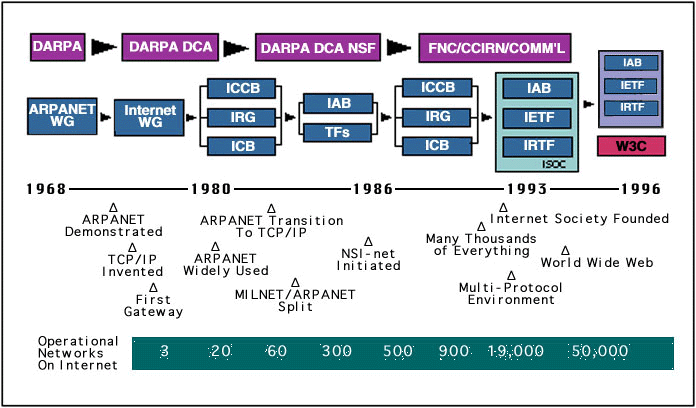
\includegraphics[width=0.8\textwidth]{images/TimelineOfTheInternetProtocols.png}
      \caption[Evolución de los protocolos de Internet]{Evolución de los protocolos de Internet. Fuente \cite{leinerBriefHistoryInternet1999}}
\end{figure}

Esta completa adopción del protocolo se dió por finalizada cuando ARPANET precursor de
internet y financiado por la Agencia de Proyectos de Investigación Avanzados de Defensa
(DARPA), llevó a cabo la transición exitosa de su antiguo protocolo, el Network Control Program
(NCP), a TCP/IP el 1 de enero de 1983 \cite{leinerBriefHistoryInternet1999}.

En resumen, la rápida adopción de la comunidad científica y académica, sumada al respaldo gubernamental consolidaron TCP/IP como el estándar dominante en la industria de las redes de comunicación.

\subsection{La World Wide Web y HTTP}
El modelo TCP/IP asentó una forma de comunicación estándar entre computadores y redes, aunque
este estaba limitado principalmente al mundo académico y científico. No fue hasta la creación de la World Wide Web (WWW)
cuando el Internet concebido como es en la actualidad se convirtió en un fenómeno global y accesible para todo el mundo.

Antes de la WWW, el acceso a la información en Internet se realizaba a través de los protocolos a nivel de aplicación mostrados en la figura \ref{fig:evolucion-protocolos}

\begin{table}[h]
      \small
      \centering
      \begin{tabular}{>{\raggedright}m{3cm}m{10cm}}
            \toprule
            \textbf{Protocolo}                                   & \textbf{Descripción}                                                                                                                                                \\
            \midrule
            FTP (Protocolo de Transferencia de Archivos)         & Utilizado para transferir archivos entre cliente y servidor a través de una red.                                                                                    \\
            \addlinespace
            Telnet                                               & Basado en texto utilizado para el acceso remoto a computadoras y servidores, permitiendo a los usuarios controlarlos a través de una interfaz de línea de comandos. \\
            \addlinespace
            Gopher                                               & Diseñado para buscar y recuperar documentos de manera jerárquica, utilizando una interfaz basada en menús.                                                          \\
            \addlinespace
            SMTP (Protocolo Simple de Transferencia de Correo)   & Utilizado para enviar mensajes de correo electrónico entre servidores y, finalmente, al cliente de correo del destinatario.                                         \\
            \addlinespace
            NNTP (Protocolo de Transferencia de Noticias en Red) & Utilizado para la distribución, consulta y recuperación de artículos de noticias en la red Usenet.                                                                  \\
            \addlinespace
            POP3 (Protocolo de Oficina de Correos 3)             & Utilizado para recuperar mensajes de correo electrónico desde un servidor de correo remoto hasta un cliente de correo local.                                        \\
            \addlinespace
            IMAP (Protocolo de Acceso a Mensajes de Internet)    & Permite a los usuarios acceder y administrar sus mensajes de correo electrónico en un servidor de correo, sin descargarlos a un cliente de correo local.            \\
            \bottomrule
      \end{tabular}
      \caption{Protocolos de capa de aplicación antes de HTTP}
      \label{fig:evolucion-protocolos}
\end{table}

Estos servicios se encuentran en nivel de aplicación dentro del \textit{stack} TCP/IP, como se muestra en la figura \ref{fig:tcpip}.
Algunos de ellos se siguen usando hoy en día, o tienen su caso de uso (IMAP, POP3, FTP), pero en lo referente a archivos,
ofrecían métodos básicos de navegación y compartición. Carecían de la capacidad de inter-conectar documentos de manera intuitiva y visual.
\footnote{Cabe destacar que en esta época, los documentos eran principalmente texto plano, sin formato, y no existía la posibilidad de incluir imágenes o vídeos.}

\usetikzlibrary{shapes,arrows,positioning, babel}
\begin{figure}[h!]
      \centering
      \begin{tikzpicture}
            % Estilos
            \tikzstyle{layer}=[draw, rectangle, minimum height=1cm, minimum width=5cm, text centered]
            \tikzstyle{app_protocol}=[draw, rectangle, minimum height=0.5cm, minimum width=1.5cm, text centered, fill=blue!10]
            \tikzstyle{arrow}=[->,>=stealth, thick]

            % Nodos
            \node[layer] (application) {Capa de aplicación};
            \node[layer, below=0.5cm of application] (transport) {Capa de transporte};
            \node[layer, below=0.5cm of transport] (network) {Capa de red};
            \node[layer, below=0.5cm of network] (link) {Capa de enlace de datos};

            \node[app_protocol, above=1cm of application.north] (imap) {IMAP};
            \node[app_protocol, left=0.2cm of imap] (pop3) {POP3};
            \node[app_protocol, right=0.2cm of imap] (nntp) {NNTP};
            \node[app_protocol, left=0.2cm of pop3] (smtp) {SMTP};
            \node[app_protocol, right=0.2cm of nntp] (gopher) {Gopher};
            \node[app_protocol, left=0.2cm of smtp] (telnet) {Telnet};
            \node[app_protocol, right=0.2cm of gopher] (ftp) {FTP};

            % Flechas
            \draw[arrow] (imap.south) -- (application.north);
            \draw[arrow] (pop3.south) -- (application.north);
            \draw[arrow] (nntp.south) -- (application.north);
            \draw[arrow] (smtp.south) -- (application.north);
            \draw[arrow] (gopher.south) -- (application.north);
            \draw[arrow] (telnet.south) -- (application.north);
            \draw[arrow] (ftp.south) -- (application.north);
      \end{tikzpicture}
      \caption{Capas del protocolo TCP/IP mostrando algunos protocolos de la capa de aplicación}
      \label{fig:tcpip}
\end{figure}

En 1989, el científico británico Tim Berners-Lee propuso la creación de la WWW, un sistema de información
global que permitiría a los usuarios navegar y acceder a documentos interconectados mediante
enlaces. Estos documentos, conocidos como páginas web, se almacenarían en computadoras conectadas a la red y podrían ser accedidos
a través de un programa especial llamado navegador web, que interpretaría el código de las páginas y mostraría su contenido al usuario.
\\HTML (Hyper Text Markup Language) es el lenguaje que describe estos documentos. Permite enlazar documentos entre sí mediante hipervínculos. Un hipervínculo es una referencia unidireccional en un documento electrónico que entrelaza diferentes documentos o secciones entre sí. Los usuarios tienen la oportunidad de seguir estos enlaces con tan solo un clic en el texto ancla (texto enlazado) para navegar a los documentos o las secciones correspondientes\cite{Hiperenlace2023}.
Aunque es un concepto simple y con el que cualquier persona en la actualidad esta familiarizada este factor dictamina la forma
en la que se usa internet en la actualidad. Los usuarios de internet interactúan con el contenido en internet mediante estos enlaces.
\\La WWW se basó en tres tecnologías clave: HTML, un lenguaje de marcado para crear páginas web; HTTP, un protocolo para solicitar y transferir recursos a través de la web; y URL, un sistema de direcciones para localizar recursos en la web\cite{leinerBriefHistoryInternet1999}. Y es este último el que genera una gran problemática que resuelve IPFS.

URL significa Uniform Resource Locator, que se traduce al español como Localizador Uniforme de Recursos. Es un sistema de direcciones utilizado en la web para localizar de manera única recursos como páginas web, imágenes, videos y otros archivos. Una URL consta de varios componentes, incluyendo el esquema (como 'http://' o 'https://'), el nombre de dominio (como 'www.ejemplo.com'), la ruta del recurso y otros parámetros opcionales.

\setlength{\parskip}{10pt}
Sin embargo, a medida que la web ha crecido en tamaño y complejidad, el enfoque de direccionamiento basado en la ubicación física
de los servidores puede presentar limitaciones. Por ejemplo, si un recurs' se encuentra en una URL específica y esa URL cambia o
el servidor deja de estar disponible, el acceso al recurso se verá comprometido.

IPFS aborda este problema mediante el uso de un sistema de direccionamiento basado en el contenido, en lugar de la ubicación. En
IPFS, cada archivo y bloque de datos se identifican mediante su contenido, utilizando una función hash criptográfica. Esto
permite que los archivos y bloques se puedan encontrar y acceder de forma fiable, independientemente de su ubicación física.

Esto permite a IPFS ofrecer una serie de ventajas sobre el sistema de direccionamiento basado en la ubicación de la web
tradicional, como la resistencia a la censura, la persistencia de los datos y la verificabilidad del contenido.
En la siguiente sección se profundizará en estas ventajas y en cómo IPFS las hace posibles.

\section{IPFS como alternativa a HTTP}\label{sect:ipfs}

\subsection{Introducción}
% Briefly introduce the concept of IPFS and its significance in the modern era of the internet.
% Provide a background on why IPFS was created and its aims.
IPFS fue presentado al mundo en 2014 por Juan Benet, en un informe técnico titulado
\textit{IPFS - Content Addressed, Versioned, P2P File System}\cite{benetIPFSContentAddressed2014}.
Benet presenta el concepto de IPFS y su proposición de crear un sistema de archivos
distribuido y descentralizado que permita a los usuarios almacenar y compartir archivos de forma segura y confiable.

Benet es también el fundador de Protocol Labs\cite{ProtocolLabs}, una empresa dedicada a la creación de protocolos de código abierto para la Web3.
IPFS es un proyecto de código abierto y, pese a que Protocol Labs está detrás de este, no es el único contribuidor a su desarrollo. Esto es otro
de los puntos fuertes de IPFS, la comunidad que lo rodea.   En la sección \ref{sect:ecosistema}: '\nameref{sect:ecosistema}' se profundiza en este aspecto.

En IPFS, cada archivo se identifica de manera única a través de su contenido mediante un hash criptográfico. Esto significa que
cualquier nodo en la red puede actuar como un proveedor de contenido al almacenar y compartir archivos, permitiendo una mayor
disponibilidad y un internet verdaderamente descentralizado. En lugar de depender de un único servidor web para acceder a un
recurso, los usuarios pueden obtener el contenido de cualquier nodo que tenga ese recurso en particular.

Estos identificadores de contenido se conocen como CID (Content Identifier). Dado que un CID es un puntero que señala a un contenido particular, se puede usar un CID en vez de URL en un enlace. De esta manera
se puede acceder a un recurso de manera fiable, independientemente de su ubicación física, mientras haya algún otro nodo de la red en posesión del
contenido que buscamos.

\subsection{Fundamentos}\label{sect:fundamentos}
% Describe the key concepts and terminologies involved in IPFS, such as Content-addressed, Peer-to-peer (P2P) network, and Merkle DAG.
% Explain how these concepts work together to make IPFS a decentralized and distributed file system.
IPFS opera a través de tres principios fundamentales que marcan una diferencia significativa con respecto a los sistemas de archivos convencionales: direccionamiento por contenido, red peer-to-peer y el grafo acíclico dirigido de Merkle (Merkle DAG).


\textbf{Direccionamiento por Contenido:} En IPFS, los archivos no se ubican por su dirección sino por su contenido. Cada archivo posee un
identificador único, denominado CID (Content Identifier), generado a partir de un hash criptográfico de su contenido. Esta característica
asegura la inmutabilidad de los archivos, es decir, los archivos no pueden ser alterados sin modificar su CID. Adicionalmente, el
direccionamiento por contenido favorece la deduplicación, dado que archivos con contenido idéntico compartirán el mismo CID, lo que conlleva a
su almacenamiento único dentro de la red.

\begin{figure}[H]
      \begin{minted}[fontsize=\small]{bash}
$ ipfs add somefile # comando para añadir archivos a ipfs a través de la línea de comandos
added QmVtuHo6C7NUonYTYUNbmgGxvSwrTVGXuahJxhxnoSxPpM somefile
      \end{minted}
      \caption{Ejemplo de CID generado por IPFS}
      \label{fig:ipfs-add}
\end{figure}

\textbf{Red Peer-to-Peer:} IPFS se basa en una red descentralizada en la que cada integrante, o nodo, puede interactuar directamente con cualquier otro nodo, sin la necesidad de intermediarios o servidores centrales. Los nodos funcionan tanto como proveedores como consumidores de contenido, guardando y compartiendo fragmentos de archivos con otros nodos. Esta red peer-to-peer hace que el contenido sea más accesible y resistente a la censura, al evitar la existencia de un único punto de fallo o control.
\begin{figure}[H]
      \centering
      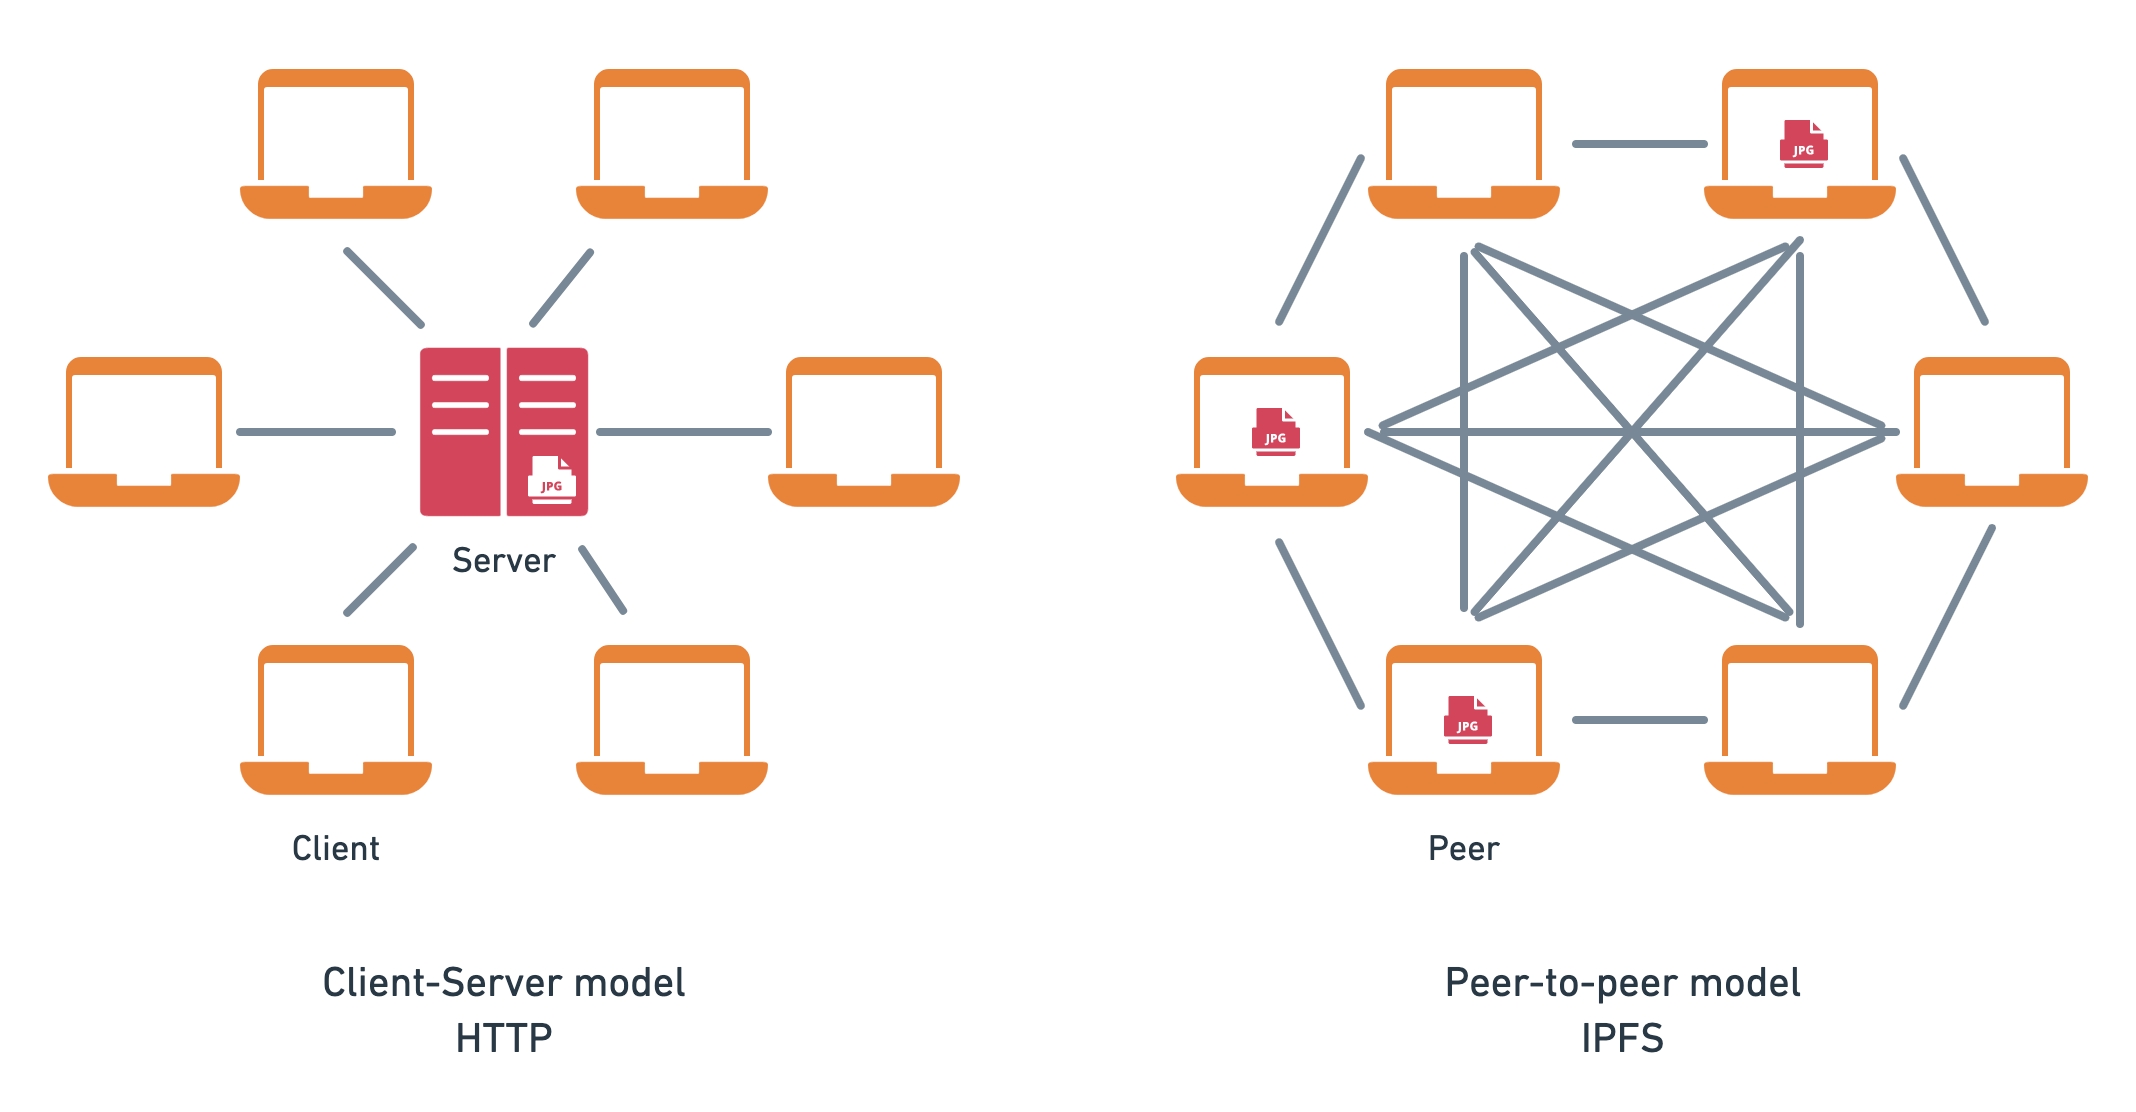
\includegraphics[width=\linewidth]{images/centralvsdecentral.png}
      \caption{Red centralizada en comparación con una red descentralizada}
      \label{fig:centralvsdecentral}
\end{figure}

\textbf{Grafo Acíclico Dirigido de Merkle (Merkle DAG):} Los archivos y sus relaciones dentro de IPFS se representan mediante una estructura de datos conocida como Merkle DAG. Un Merkle DAG es un grafo donde cada nodo tiene un identificador único (CID) que se genera a partir de su contenido y el de sus nodos hijos. Los nodos pueden ser hojas o nodos intermedios, dependiendo de si tienen o no nodos hijos. Los nodos hoja contienen datos binarios de los archivos, mientras que los nodos intermedios contienen enlaces a otros nodos. Los nodos intermedios permiten dividir archivos grandes en bloques más pequeños y formar estructuras jerárquicas, como directorios o sistemas de archivos. El Merkle DAG facilita la verificación de integridad y autenticidad de los archivos, dado que cualquier cambio en el contenido o en los enlaces se refleja en el CID del nodo afectado y sus ancestros.

Cada uno de estos conceptos se profundizará dentro del apartado correspondiente a continuación.

\subsection{Arquitectura}
% Describe the core components of IPFS architecture, such as IPFS node, IPFS client, IPFS gateway, and IPFS cluster.
% Explain the role of each component in the IPFS network.
IPFS es un conjunto de protocolos de código abierto que combina múltiples conceptos existentes de redes
peer-to-peer (P2P), datos enlazados y otras áreas para permitir que los participantes intercambien fragmentos de
archivos.

Estos conceptos concretados en protocolos forman distintos niveles de abstracción, cada uno de los cuales se puede utilizar de forma independiente y conforman la arquitectura de IPFS, también conocido como el \textit{stack} de protocolos de IPFS. En la figura \ref{fig:ipfs} se muestra el stack de protocolos de IPFS.

\begin{figure}[H]
      \centering
      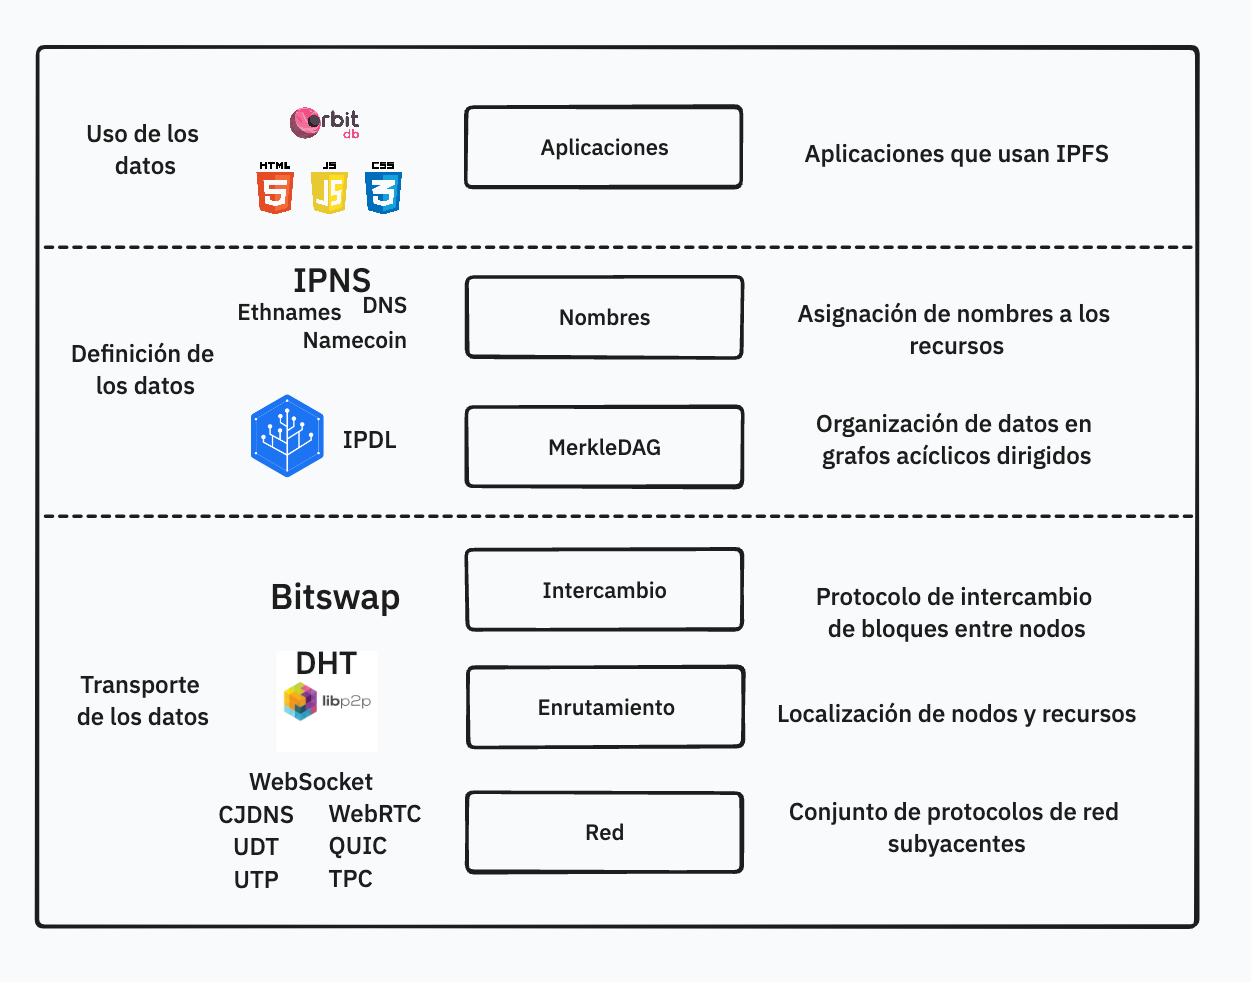
\includegraphics[width=\linewidth]{images/ipfs-stack.png}
      \caption{Stack de protocolos IPFS}
      \label{fig:ipfs}
\end{figure}

Como se puede observar, este stack se divide tres grupos según la funcionalidad que brinda cada capa.
Este diseño en capas subdivido en componentes independientes permite que estos pueden ser ampliados o reemplazados
según se necesite. Esta modularidad en el diseño está respaldada por una biblioteca de redes P2P llamada libp2p\cite{WhatLibp2p}.

Libp2p es una suite de protocolos y herramientas modulares que permite la creación de sistemas de red peer-to-peer (P2P). Se encarga de gestionar todas las necesidades de red, como la negociación de protocolos, el enrutamiento, la detección de nodos y la transmisión de datos.

\subsubsection{Capa de red}
En la capa de red encontramos los protocolos de transporte de red mediante los cuales los nodos se pueden comunicar. Estos protocolos provienen de libp2p\cite{labsLibp2pConnectivity} y son los siguientes:
\begin{itemize}[itemsep=1pt,nolistsep]
      \item \textbf{TCP}: proporciona una entrega de datos confiable, ordenada y con control de errores sobre redes IP.
      \item \textbf{UDP}: proporciona una entrega de datos simple, sin conexión y no confiable sobre redes IP.
      \item \textbf{QUIC}: Un protocolo de transporte multiplexado y seguro que se ejecuta sobre UDP, proporcionando flujos confiables, de baja latencia y cifrados.
      \item \textbf{WebSockets}: Un protocolo que permite la comunicación bidireccional entre un navegador web y un servidor sobre TCP.
      \item \textbf{WebRTC}: Un protocolo que permite la comunicación en tiempo real entre navegadores web mediante conexiones peer-to-peer.
\end{itemize}

Debido a esta gran variedad de protocolos de transporte, libp2p proporciona una forma de identificar el transporte que se esté usando mediante
direcciones \textit{multiaddr}.
Los multiaddresses son una forma de representar las direcciones de red como encapsulaciones de protocolos arbitrarios. Estos multiaddresses admiten direccionar
para cualquier protocolo de red. Siguen una sintáxis  simple, lo que los hace fáciles de analizar y construir.

En IPFS, se utilizan los multiaddresses para identificar y localizar los nodos en la red. Cada nodo al configurarse por primera vez
genera un par de claves pública y privada. La clave pública se utiliza para crear un identificador único del nodo en la red llamado peerID, que es el hash de su esta clave pública. La clave privada se utiliza para firmar mensajes y autenticar la identidad del nodo. Además, los nodos tienen una o más direcciones de red que combinan protocolos y valores para indicar cómo conectarse a ellos. Por ejemplo, una dirección de red podría ser /ip4/1.2.3.4/tcp/4001/ipfs/QmFoo, lo que significa que el nodo QmFoo está escuchando conexiones TCP en el puerto 4001 utilizando la dirección IP 1.2.3.4.

Los multiaddresses se pueden encapsular entre sí para crear capas de transporte más complejas. Por ejemplo, se puede utilizar /dns4/example.com/tcp/1234/tls/ws/tls para indicar una conexión segura con WebSockets sobre TLS utilizando el dominio example.com y el puerto 1234.

La amplia variedad de protocolos de transporte disponibles garantiza la adaptabilidad de IPFS, ya que los nodos pueden utilizar múltiples protocolos de transporte simultáneamente y cambiar entre ellos según las condiciones de la red. Esto significa que las opciones de transporte de un nodo dependen del entorno en el que se ejecute. Por ejemplo, en un navegador web sólo se pueden utilizar WebSockets y WebRTC, mientras que en otros entornos se pueden utilizar todos los protocolos mencionados anteriormente, siempre que sean compatibles a nivel de sistema operativo y hardware.

\subsubsection{Enrutamiento y descubrimiento de nodos}
\textbf{Descubrimiento de nodos:}
\\Es el proceso de encontrar y anunciar servicios a otros nodos en una red P2P. Se puede realizar utilizando diversos protocolos,
como por ejemplo, la difusión de mensajes a todos los nodos de la red o utilizar una serie nodo de arranque para proporcionar una lista de nodos conocidos.

Esto último se conoce como nodos de arranque (bootstrapping). Es una lista de nodos predefinidos  y de confianza que ayudan a los nuevos nodos a unirse a la red y a descubrir otros nodos, facilitando el proceso de construcción y mantenimiento de la red distribuida. La lista de bootsrappers la define cada nodo. La figura \ref{fig:ipfsbootsrapper} muestra los bootstrappers por defecto en una instalación de IPFS.

\begin{figure}[H]
      \centering
      \small
      \begin{minted}{json}
"Bootstrap": [
"/dnsaddr/bootstrap.libp2p.io/p2p/QmNnooDu7bfjPFoTZYxMNLWUQJyrVwtbZg5gBMjTezGAJN",
"/dnsaddr/bootstrap.libp2p.io/p2p/QmQCU2EcMqAqQPR2i9bChDtGNJchTbq5TbXJJ16u19uLTa",
"/dnsaddr/bootstrap.libp2p.io/p2p/QmbLHAnMoJPWSCR5Zhtx6BHJX9KiKNN6tpvbUcqanj75Nb",
"/dnsaddr/bootstrap.libp2p.io/p2p/QmcZf59bWwK5XFi76CZX8cbJ4BhTzzA3gU1ZjYZcYW3dwt",
"/ip4/104.131.131.82/tcp/4001/p2p/QmaCpDMGvV2BGHeYERUEnRQAwe3N8SzbUtfsmvsqQLuvuJ",
"/ip4/104.131.131.82/udp/4001/quic/p2p/QmaCpDMGvV2BGHeYERUEnRQAwe3N8SzbUtfsmvsqQLuvuJ"
],
      \end{minted}
      \caption{Bootstrappers por defecto en una instalación de IPFS}
      \label{fig:ipfsbootsrapper}
\end{figure}

\textbf{Enrutamiento}:
\\Por otro lado, enrutamiento se refiere a encontrar la ubicación específica de otro nodo de la red. Esto se realiza
típicamente mediante el mantenimiento de una tabla de enrutamiento u otra estructura de datos similar que realiza un
seguimiento de la topología de la red. En el caso de IPFS se usa una tabla de hash distribuida conocida como DHT (Distributed
hash table).

En la práctica, la distinción entre el enrutamiento y el descubrimiento de nodos no siempre está clara, de hecho suelen ocurrir simultáneamente.

Los protocolos principales\footnote{Existen más protocolos de enrutamiento y descubrimiento de nodos en libp2p pero estos son los más utilizados por IPFS.} que usa IPFS y libp2p para este propósito son:

\begin{itemize}[itemsep=1pt,nolistsep]
      \item \textbf{ping}: Protocolo de comprobación de disponibilidad. Los nodos pueden utilizarlo para verificar la conectividad y el rendimiento entre ellos.
      \item \textbf{autonat}: Protocolo de detección de NAT. Asiste a los nodos en la identificación de su accesibilidad desde internet, esto es útil para detectar si los nodos que se encuentran ocultos detrás de un NAT o de un firewall \cite{AutoNAT}.
      \item \textbf{identify}: Protocolo para el intercambio de claves y direcciones con otros nodos. Facilita el intercambio de información esencial, como los protocolos soportados, las claves públicas, las direcciones, etc.
      \item \textbf{kademlia}: Protocolo para la implementación de una tabla hash distribuida para el almacenamiento descentralizado y la recuperación de información de nodos y contenidos.
      \item \textbf{mdns}: Protocolo de descubrimiento de nodos locales con cero configuración, usando DNS de multidifusión. Ofrece un mecanismo para que los nodos en la misma red local se descubran entre sí sin configuración previa.
      \item \textbf{Circuit Relays}: Es un protocolo que facilita a los nodos el reenvío de tráfico en nombre de otros nodos que no tienen un acceso directo entre ellos\cite{CircuitRelay}.
      \item \textbf{rendezvous}: Un protocolo de encuentro que se utiliza como un punto común entre dos rutas.
            Los puntos de encuentro son típicamente nodos que están bien conectados y son estables en una red, y pueden manejar grandes cantidades de tráfico y datos. Sirven como un centro para que los nodos se descubran. De los pocos mecanismos centralizados que usa libp2p \cite{Rendezvous}.
      \item \textbf{pubsub}: Es una interfaz PubSub para libp2p, diseñada para establecer una base para la comunicación de mensajes mediante un patrón de publicación y suscripción entre los nodos de la red libp2p. Existen diferentes implementaciones de este protocolo, como FloodSub, GossipSub que proporcionan
            diferentes ventajas.
\end{itemize}

Tal como se indicó previamente, libp2p dispone de varias estrategias para el enrutamiento y la detección de nodos. IPFS las utiliza todas en sus diferentes configuraciones. La elección de la combinación de estas estrategias se realiza en función del contexto particular de un nodo respecto de
otros nodos y la red.

\subsubsection{Mecanismo de intercambio de contenido}

\textbf{Bitswap:} Es un protocolo de intercambio de contenido que se ejecuta sobre una red P2P. Bitswap permite a los nodos intercambiar bloques de datos entre los nodos que conforman la red. Estos pueden solicitar bloques de datos a otros nodos y compartir los bloques que disponen. Bitswap utiliza un mecanismo de intercambio de deuda para
garantizar que los nodos intercambien bloques de datos de manera justa y equitativa.
Todo esto es posible gracias a que Bitswap mantiene un registro de los bloques que cada nodo tiene y los bloques que necesita.

La transferencia de datos (bloques) en IPFS está inspirada en BitTorrent, pero no es igual uno a uno comparado con este. Dos características de BitTorrent que utiliza IPFS:
\begin{itemize}[itemsep=1pt,nolistsep]
      \item Estrategia de tit-for-tat (el que no comparte no recibe).
      \item Obtén primero las piezas raras (mejora el rendimiento).
\end{itemize}
Una diferencia notable es que en BitTorrent cada archivo tiene un enjambre (también conocido como \textit{swarm}) separado de nodos (formando una red P2P entre ellos). En cambio, IPFS es una única red de nodos formando un gran swarm. La variedad de BitTorrent en IPFS es el ya mecionado Bitswap.

Bitswap es el algoritmo de intercambio de bloques, pero para realizar este intercambio primero se debe saber qué nodos pueden proveer los bloque que se buscan.
Esto es posible gracias a la DHT. En IPFS la DHT se utiliza principalmente con dos funciones:
% enumerated list with numbers
\begin{enumerate}
      \item \textbf{Enrutamiento:} se ha explicado en la subsección anterior.
      \item \textbf{Anuncios de provisión/consumición de contenido:} los nodos publican en la DHT los bloques de datos que tienen disponibles. Esto permite a otros nodos saber quién tiene los bloques de datos que están buscando. Esta tabla de hash se distribuye por la red mediante el algoritmo de Kademlia.
\end{enumerate}

Sobre el segundo, que es el concierne dentro del mecanismo de intercambio de contenido: Cada nodo tiene dos lista de bloques (CIDs). Bloques que posee y puede
proporcionar, y bloques que desea obtener.
\begin{itemize}[itemsep=1pt]
      \item Al recibir una lista de deseos, una entidad que use Bitswap debería procesarla eventualmente y responder al solicitante con información sobre el bloque o el bloque en sí.
      \item Al recibir bloques, el nodo consumidor debe enviar una notificación de cancelación al resto de nodos a los que ha pedido estos bloques, señalando que  ya no los desea.
\end{itemize}


\begin{figure}[H]
      \centering
      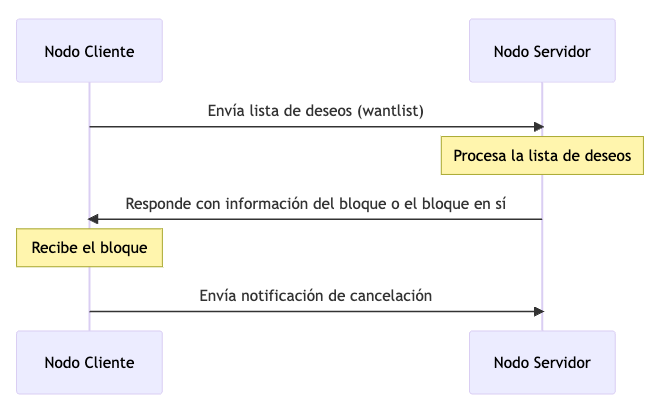
\includegraphics[width=0.8\textwidth]{images/bitswap.png}
      \caption{Protocolo Bitswap}
      \label{bitswap}
\end{figure}


Por último cabe destacar un concepto muy importante dentro de IPFS en torno al guardado de bloques:
\textbf{la recolección de basura.}

Cada nodo tiene una capacidad
de almacenamiento, siendo esta el límite de bloques que puede almacenar. A medida que un nodo va obteniendo y compartiendo más
contenido a través de IPFS, los bloques que recibe se van ubicando su almacenamiento local. La cantidad de bloques puede aumentar
rápidamente y ocupar espacio innecesario. Algunos de estos bloques pueden estar referenciados por objetos obsoletos o que ya no son
necesarios, lo que significa que no se utilizan ni se acceden directamente.

La recolección de basura en IPFS es el proceso mediante el cual se eliminan los bloques que ya no son necesarios en un nodo. Sin embargo, IPFS utiliza un sistema de almacenamiento basado en referencias, lo que significa que un bloque puede ser referenciado por múltiples objetos y mantenerse en el sistema aunque no esté directamente en uso.

Para evitar que los bloques necesarios sean eliminados por accidente sin el deseo del usuario poseedor del nodo, IPFS introduce el concepto de \textit{pinning}. Un pin es una
instrucción que le indica al nodo que debe mantener un bloque o conjunto de bloques en su almacenamiento local, incluso si no están
siendo utilizados directamente por el nodo.

Los pinsets son conjuntos de CIDs que se desean mantener en el nodo. Estos pinsets permiten a los usuarios
especificar qué bloques desean mantener de manera persistente, evitando así que sean eliminados durante el proceso de
recolección de basura.

En resumen, los pinsets son conjuntos de CIDs que representan bloques que un nodo desea mantener en su almacenamiento local, y utilizan el concepto de 'pins' para asegurarse de que estos bloques no sean eliminados accidentalmente durante la recolección de basura.

\subsection{Modelo de datos}\label{sect:modelo-de-datos}
\subsubsection{DAG de Merkle}
El modelo de datos en IPFS está basado en árboles de Merkle. Es una estructura de datos en la que cada nodo es una representación hash de un conjunto de datos.
Los nodos hoja son representaciones (generalmente a través de una función de hash) de bloques de datos, mientras que cada nodo interno es la representación
(nuevamente, generalmente a través de una función de hash) de sus nodos hijos. Esto crea un sistema en el que cualquier cambio en los datos originales cambiará
los hashes en la ruta hasta la raíz del árbol, proporcionando una forma de verificar la integridad de los datos.

Un DAG de Merkle es una estructura donde cada nodo es un árbol de Merkle, y están conectados formando un grafo acíclico direccionado.
Esto significa que los nodos están conectados de tal manera que siempre hay una dirección (de nodos padres a nodos hijos) y no hay ciclos (no puedes empezar en un nodo, seguir las conexiones y volver al nodo original).

\begin{figure}[H]
      \centering
      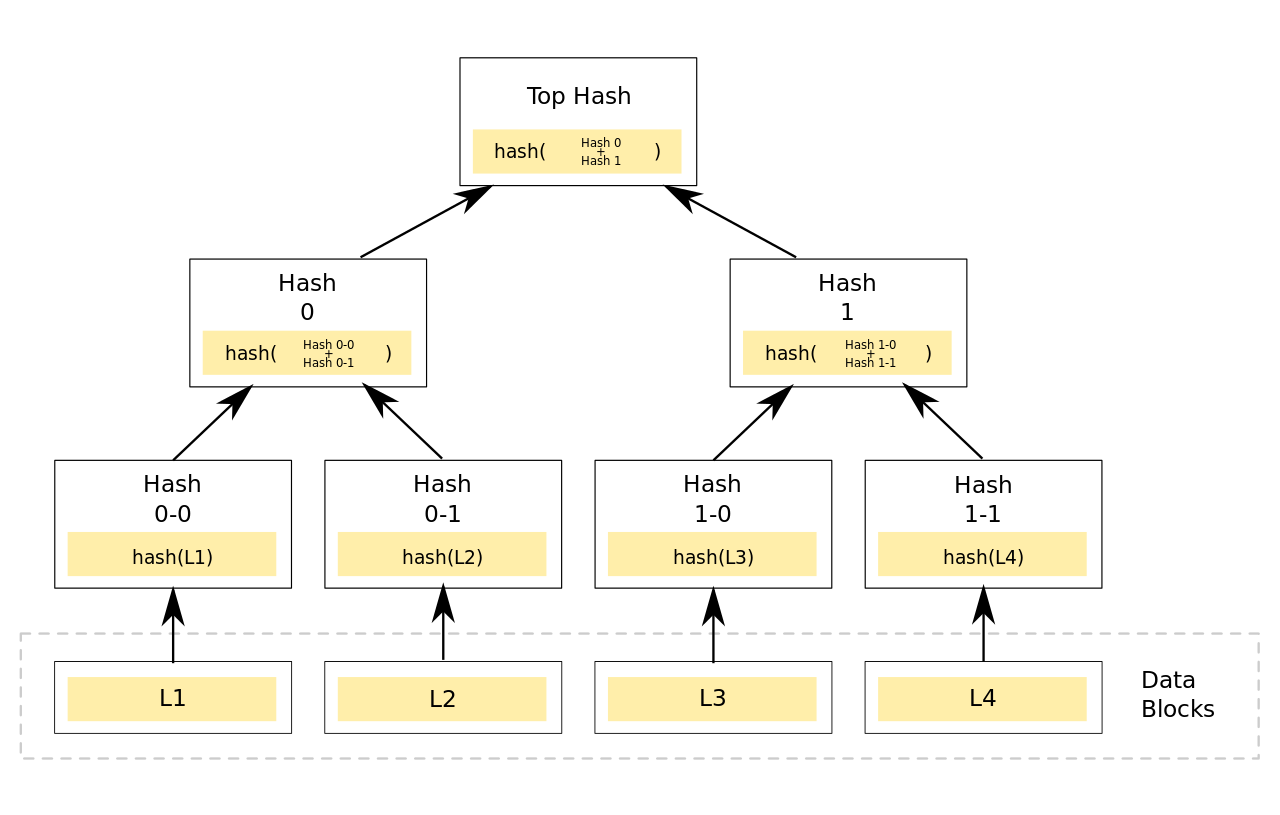
\includegraphics[width=0.8\textwidth]{images/merkledag.png}
      \caption{Ejemplo de un árbol de Merkle}
      \label{merkledag}
\end{figure}

\subsubsection{IPLD}
IPLD (InterPlanetary Linked Data)\cite{IPLDDocs} es un estructura basada en un DAG de Merkle que permite enlazar datos entre diferentes sistemas
distribuidos, como IPFS, Bitcoin o Ethereum. Una estructura de datos inmutable es aquella que no puede ser modificada una vez creada, lo que ofrece
ventajas como la seguridad, la consistencia y la ausencia de efectos secundarios. IPLD utiliza estructuras de datos inmutables para representar los
bloques de datos que se almacenan y se enlazan entre sí mediante CIDs.

IPLD es una capa de abstracción que permite a los desarrolladores trabajar con datos en diferentes plataformas y protocolos como si estuvieran trabajando con un solo sistema cohesivo. Permite la interoperabilidad a gran escala entre diferentes sistemas de almacenamiento de datos, lo que facilita la creación de aplicaciones y servicios más robustos y resistentes en entornos distribuidos.

El DAG también garantiza a IPFS con característica de control de versiones como Git. Aunque este es un apartado en el que se profundiza poco en IPFS.
En el whitepaper, Benet se refiere más bien al hecho de que al igual que Git, IPFS usa Merkle DAGs, y por lo tanto posee características de
control de versiones. Los nodos en un Merkle DAG son inmutables. Cualquier cambio en un nodo alteraría su identificador y, por lo tanto, afectaría a
todos los ascendentes en el DAG, creando esencialmente un DAG diferente.

En lo que respecta a este trabajo, este hecho permite la propia existencia de OrbitDB, el cual es una pieza clave en el desarrollo de este proyecto. OrbitDB implementa bases de datos distrubuidas en IPFS, se basa en este concepto al ser los datos inmutables y permitir la reconstrucción de la base de datos mediante el intercambio de objetos y la actualización de referencias remotas.
TODO poner referencia a orbitdb

\subsubsection{Códecs de IPLD}

Los códecs de IPLD son funciones que transforman el modelo de datos de IPLD en bytes serializados para que puedas enviar y compartir datos, y transforman los
bytes serializados de nuevo en el modelo de datos de IPLD para que puedas trabajar con él. Algunos de estos códecs incluyen:

\begin{itemize}[itemsep=1pt,nolistsep]
      \item \textbf{DAG-CBOR:} es un formato binario que soporta el modelo de datos de IPLD al completo. Ofrece un excelente rendimiento y es adecuado para cualquier tipo de trabajo.
      \item \textbf{DAG-JSON:} está basado en JSON (Javascript Object Notation). Es un formato más legible, lo que lo hace muy conveniente para la interoperabilidad, el desarrollo y a la hora de depurar código que haga uso de IPLD.
      \item \textbf{DAG-PB:} es otro formato binario usado principalmente para serializar datos en fornmato de unixfsv1 (ir a \ref{subsect:unixfs}: '\nameref{subsect:unixfs}' para más información).
      \item \textbf{DAG-JOSE:} El codec dag-jose es un formato para firmar y cifrar objetos JSON.
\end{itemize}

En este proyecto se ha hecho especial incapié en el uso de DAG-JOSE como códec de los datos en el DAG de Merkle. Esto permite la firma y cifrado de
en objetos JWS (JSON Web Signatures) y JWE (JSON Web Encryption) representados en nodos del DAG de IPLD.
TODO poner referencia a la parte de JWE y JWS

\subsubsection{Unixfs}\label{subsect:unixfs}
Sobre todo este modelo de datos se establecen otras estructura o abstracciones como Unixfs.

Cuando se agrega un archivo a IPFS, puede que sea demasiado grande para caber en un solo bloque, por lo que se divide en disintos bloques que luego son
representados mediante metadatos en una lista de enlaces a estos bloques. UnixFS es un formato usado para describir archivos, directorios y enlaces simbólicos en
IPFS. Este formato de datos se usa para representar archivos y todos sus enlaces y metadatos en IPFS. UnixFS crea un bloque (o un árbol de bloques) de objetos enlazados.

\begin{minted}[fontsize=\small]{bash}
$ ipfs add Pictures/Wallpapers/ -r
added QmT4pCxAKwjKz58FRkKGZUkuk9dBogzvSqfKaP9aXxRsLh Wallpapers/flow 1.jpg
added QmY1KMKAoHmDK9V3woMGGarVUJ4a1a4HCW1CxRXMtC9KwP Wallpapers/flow 2.jpg

added QmYmdHatxVXfSy9Gjdp8e75cL2mvsGyZ1tT6Qo3ijUV2h5 Wallpapers
\end{minted}

Al obervar el contenido del CID final de la carpeta subida en el DAG

\begin{minted}[fontsize=\small]{bash}
$ ipfs dag get /ipfs/QmYmdHatxVXfSy9Gjdp8e75cL2mvsGyZ1tT6Qo3ijUV2h5 | jq
\end{minted}
\begin{minted}[fontsize=\small]{json}
{
  "Data": {
    "/": {
      "bytes": "CAE"
    }
  },
  "Links": [
      {
      "Hash": {
        "/": "QmT4pCxAKwjKz58FRkKGZUkuk9dBogzvSqfKaP9aXxRsLh"
      },
      "Name": "flow 1.jpg",
      "Tsize": 50087191
    },
    {
      "Hash": {
        "/": "QmVRXnTfUDxioWNZ5FbA79xuiZGtkUuxL6rae1MtstGuzu"
      },
      "Name": "flow 2.jpg",
      "Tsize": 32032025
    },
  ]
}
\end{minted}

Como se puede observar el DAG contiene la estructura de datos que modela un directorio, en este caso de tipo directorio.
\begin{minted}[fontsize=\small]{bash}
$ ipfs files stat /ipfs/QmYmdHatxVXfSy9Gjdp8e75cL2mvsGyZ1tT6Qo3ijUV2h5
Size: 0
CumulativeSize: 549538133
ChildBlocks: 22
Type: directory
\end{minted}

En cambio si se observa el contenido en el DAG de uno de los archivos enlazados:
\begin{minted}[fontsize=\small]{bash}
$ ipfs dag get QmT4pCxAKwjKz58FRkKGZUkuk9dBogzvSqfKaP9aXxRsLh | jq
{
  "Data": {
    "/": {
      "bytes": "CAIYnKzwFyCAgOAVIJyskAI"
    }
  },
  "Links": [
    {
      "Hash": {
        "/": "QmbhvAYKs4ERhnvujqDdTVCZdV2Y8UqrnFjGTVver1rzFL"
      },
      "Name": "",
      "Tsize": 45623854
    },
    {
      "Hash": {
        "/": "QmRw866oefrQ98iYb71cvKMmHTLsoTUW5j2cmRR5kkRqLf"
      },
      "Name": "",
      "Tsize": 4463228
    }
  ]
}
\end{minted}
El archivo ocupa dos bloques cuyos CIDs están en la lista de enlaces del objeto.
\begin{minted}[fontsize=\small]{bash}
$ ipfs files stat /ipfs/QmT4pCxAKwjKz58FRkKGZUkuk9dBogzvSqfKaP9aXxRsLh
QmT4pCxAKwjKz58FRkKGZUkuk9dBogzvSqfKaP9aXxRsLh
Size: 50075164
CumulativeSize: 50087191
ChildBlocks: 2
Type: fil
\end{minted}

\subsubsection{MFS}

Sobre Unixfs existe otra capa más que es la que realmente permite una interacción con IPFS como si de un
sistema de ficheros tradicional se tratara. Este componente es denominado \textit{Mutable File System} (MFS) o Sistema de Archivos Mutable.
Para hacer esto posible, MFS mantiene un mapa de la estructura de archivos y directorios en IPFS. Cada vez que se realiza una operación en MFS, como crear o mover
un archivo, se actualiza este mapa. Sin embargo, los datos subyacentes en IPFS permanecen inalterados. Esto significa que se pueden cambiar la estructura y
organización de archivos y directorios en MFS sin tener que copiar o mover los datos reales, manipulando enlaces dentro del DAG.
\begin{figure}[H]
      \vspace{10pt}
      \centering
      \begin{tikzpicture}[node distance = 0.5cm, auto]
            % Estilos
            \tikzstyle{block} = [rectangle, draw, fill=blue!20,
            text width=5cm, text centered, rounded corners, minimum height=1cm]

            \node [block] (mfs) {MFS \\ Sistema de archivos};
            \node [block, below = of mfs] (unixfs) {UnixFS \\ Archivos y directorios};
            \node [block, below = of unixfs] (dag) {DAG \\ Nodos};
            \node [block, below = of dag] (block) {Bloque \\ Flujo de bits};

            \draw (mfs) -- (unixfs);
            \draw (unixfs) -- (dag);
            \draw (dag) -- (block);
      \end{tikzpicture}
      \caption{Capas de abstracción sobre los datos en IPFS}
      \label{fig:modelo-datos-ipfs}
\end{figure}


\subsection{Sistema de nombres}


IPNS, o Sistema de Nombres Interplanetario, es un componente fundamental de IPFS que permite la creación de nombres persistentes para diferentes
nodos en la red IPFS. Dado que los contenidos en IPFS son inmutables y se accede a ellos a través de sus CIDs,
cualquier cambio en el contenido dará lugar a un nuevo CID. Esto puede resultar inconveniente para los usuarios que necesitan referirse a un contenido
específico, incluso si este cambia con el tiempo. Aquí es donde entra en juego IPNS.

IPNS proporciona una capa de indirección que permite a los usuarios referirse a contenidos que pueden cambiar con el tiempo usando un nombre persistente.
En lugar de tener que actualizar el CID cada vez que cambia el contenido, los usuarios pueden referirse al contenido usando un identificador IPNS.
Este identificador es una clave criptográfica que se genera cuando se inicializa un nodo IPFS, y es única para cada nodo.

Cuando se desea publicar contenido bajo IPNS, se crea un registro que vincula el identificador IPNS con el CID del contenido.
Este registro se firma con la clave privada del nodo, garantizando que solo el propietario del identificador IPNS puede cambiar la vinculación.
El registro, contenido en la DHT se propaga luego a través de la red IPFS mediante Kademlia. Cuando otros nodos quieren acceder al contenido, pueden buscar el registro usando el identificador IPNS y obtener el CID correspondiente.

IPNS es de interés particular para este proyecto debido a que permite crear enlaces persistentes a contenido que puede cambiar con el tiempo.
Tal y como sucede con una URL que enlaza a un contenido compartido en plataformas de almacenamiento en la nube como Google Drive o Dropbox.

Este es el último apartado en esta explicación de los fundamentos de IPFS. Por supuesto, no se ha cubierto todo lo que IPFS ofrece, pero sí los
conceptos fundamentales necesarios para entender el sistema que se propone en el proyecto.

\section{Ecosistema en torno a IPFS}\label{sect:ecosistema}
\subsection{Introducción}
El ecosistema IPFS es un conjunto diverso y creciente de proyectos, herramientas, comunidades e integraciones que trabajan colectivamente para desarrollar, adoptar y evolucionar IPFS. Este ecosistema es fundamental para el éxito y la adopción generalizada de IPFS, ya que proporciona una variedad de recursos y oportunidades para interactuar y construir sobre el mismo.

\subsection{Proyectos basados en IPFS}
Existen numerosos proyectos y productos que se basan en IPFS para ofrecer soluciones innovadoras y disruptivas en diferentes áreas de aplicación. Algunas de estas áreas son:
\begin{itemize}
      \item Almacenamiento: proyectos que utilizan IPFS para proporcionar servicios de almacenamiento distribuido, persistente y rentable, como Filecoin, Sia, Storj o Textile.
      \item Alojamiento web: proyectos que utilizan IPFS para alojar sitios web estáticos o dinámicos sin depender de servidores centralizados, como Fleek, Pinata o Unstoppable Domains.
      \item Distribución de contenido: proyectos que utilizan IPFS para distribuir contenido multimedia, educativo o informativo de forma eficiente y descentralizada, como Audius, Wikipedia Mirror o Origin Protocol.
      \item Aplicaciones descentralizadas (dApps): proyectos que utilizan IPFS para construir aplicaciones web que funcionan sobre redes peer-to-peer, sin intermediarios ni puntos de fallo, como Brave, Metamask o OpenBazaar.

\end{itemize}
\subsection{Herramientas y librerías de IPFS}
Existen diversas herramientas y librerías que facilitan el desarrollo y la integración con IPFS, tanto para usuarios finales como para desarrolladores.
Algunas de estas herramientas y librerías son:
\begin{itemize}
      \item Clientes API: herramientas que permiten interactuar con un nodo IPFS a través de una interfaz de programación de aplicaciones (API), como ipfs-http-client, ipfs-js or py-ipfs-http-client.
      \item Interfaces de línea de comandos: herramientas que permiten interactuar con un nodo IPFS a través de una terminal o consola, como ipfs or ipfs-cluster.
      \item Marcos de desarrollo: herramientas que facilitan la creación y el despliegue de aplicaciones basadas en IPFS, como Fleek, Textile or 3Box.
      \item Librerías para integrar IPFS: herramientas que permiten integrar IPFS en otras aplicaciones o plataformas, como ipfs-embed, js-ipfs or go-ipfs.

\end{itemize}
\subsection{Comunidades en torno a IPFS}
Existen diversas comunidades que se forman alrededor de IPFS, tanto para apoyar el desarrollo y la adopción del proyecto, como para explorar sus posibilidades y beneficios.
Algunas de estas comunidades son:
\begin{itemize}
      \item Comunidades de desarrolladores: comunidades que se dedican a contribuir al código fuente, a reportar errores, a proponer mejoras o a crear nuevas funcionalidades para IPFS, como el equipo principal de IPFS, los colaboradores externos o los grupos locales.
      \item Comunidades de usuarios: comunidades que se dedican a utilizar IPFS para sus propios fines, a compartir experiencias, a resolver dudas o a dar feedback sobre el proyecto, como los usuarios finales, los creadores de contenido o los operadores de nodos.
      \item Comunidades de gobernancia: comunidades que se dedican a definir las reglas, los principios y los objetivos del proyecto IPFS, así como a coordinar las acciones y los recursos necesarios para su cumplimiento, como el Protocol Labs, la Fundación Filecoin o el Consejo Asesor.
\end{itemize}
\subsection{Integraciones de IPFS}
Existen diversas formas en las que IPFS se integra con otras tecnologías y plataformas para ampliar sus capacidades y su alcance.
Algunas de estas integraciones son:
\begin{itemize}
      \item Ethereum: una plataforma de computación descentralizada que permite la creación de contratos inteligentes y aplicaciones descentralizadas. IPFS se integra con Ethereum para almacenar y distribuir los datos asociados a estas aplicaciones, así como para mejorar la escalabilidad y la eficiencia de la red.
      \item Filecoin: una red de almacenamiento descentralizado que permite a los usuarios alquilar o proveer espacio de disco a cambio de una criptomoneda. IPFS se integra con Filecoin para ofrecer una capa de incentivos económicos y una garantía de disponibilidad y persistencia de los datos almacenados en IPFS.
\end{itemize}

Como se puede apreciar IPFS es un proyecto con una gran comunidad y un ecosistema muy activo. Dada su naturaleza IPFS
es un proyecto que se puede integrar en cantidad de ámbitos y tecnologías, ofreciendo las ventajas ya previamente mencionadas.

\chapter{Estado del arte}\label{chap:3estadodelarte}

En este capítulo se lleva a cabo un breve análisis de algunas implementaciones, tecnologías y plataformas que usan IPFS
y cumplen parcial o completamente con los objetivos del proyecto.

Como se ha visto en el apartado anterior existen una gran cantidad de herramientas y proyectos
que usan IPFS como base para sus sistemas. Pese a esto en el contexto de archivos compartidos, solo existen
algunos proyectos interesantes que merece la pena analizar:

\section{Peergos}

Peergos es con una plataforma web para subir archivos y compartirlos con otros usuarios. Cuenta con un sistema de
almacenamiento y comunicación descentralizado y seguro que utiliza criptografía y la red IPFS. Como se puede observar en la
figura \ref{fig:peergos} Peergos proporciona una interfaz web para guardar,
compartir y editar archivos, fotos, vídeos, mensajes y otros datos de forma privada y sin intermediarios. Peergos garantiza que
solo los usuarios autorizados puedan acceder a sus datos, y que nadie pueda espiar o censurar su actividad en línea. Es una
plataforma de código abierto y se puede ejecutar en cualquier dispositivo compatible con Java \cite{PeergosPeergosP2p}.

Este proyecto se encuentra en fase de desarrollo, aunque es un producto completo que además ofrece planes de almacenamiento
como si de un proveedor en la nube se tratara. Esto es posible ya que al ser IPFS una red global,
cualquier nodo de la red puede mantener \textit{pinneados} (disponibles) los bloques que se deseen, y por tanto
ofrecer un servicio de almacenamiento. En este caso Peergos ofrece un servicio de almacenamiento de pago, es decir,
que tienen una serie de nodos en la red que mantienen pinneados los bloques de datos de los usuarios que pagan por el servicio.

\begin{figure}[H]
    \centering
    \small
    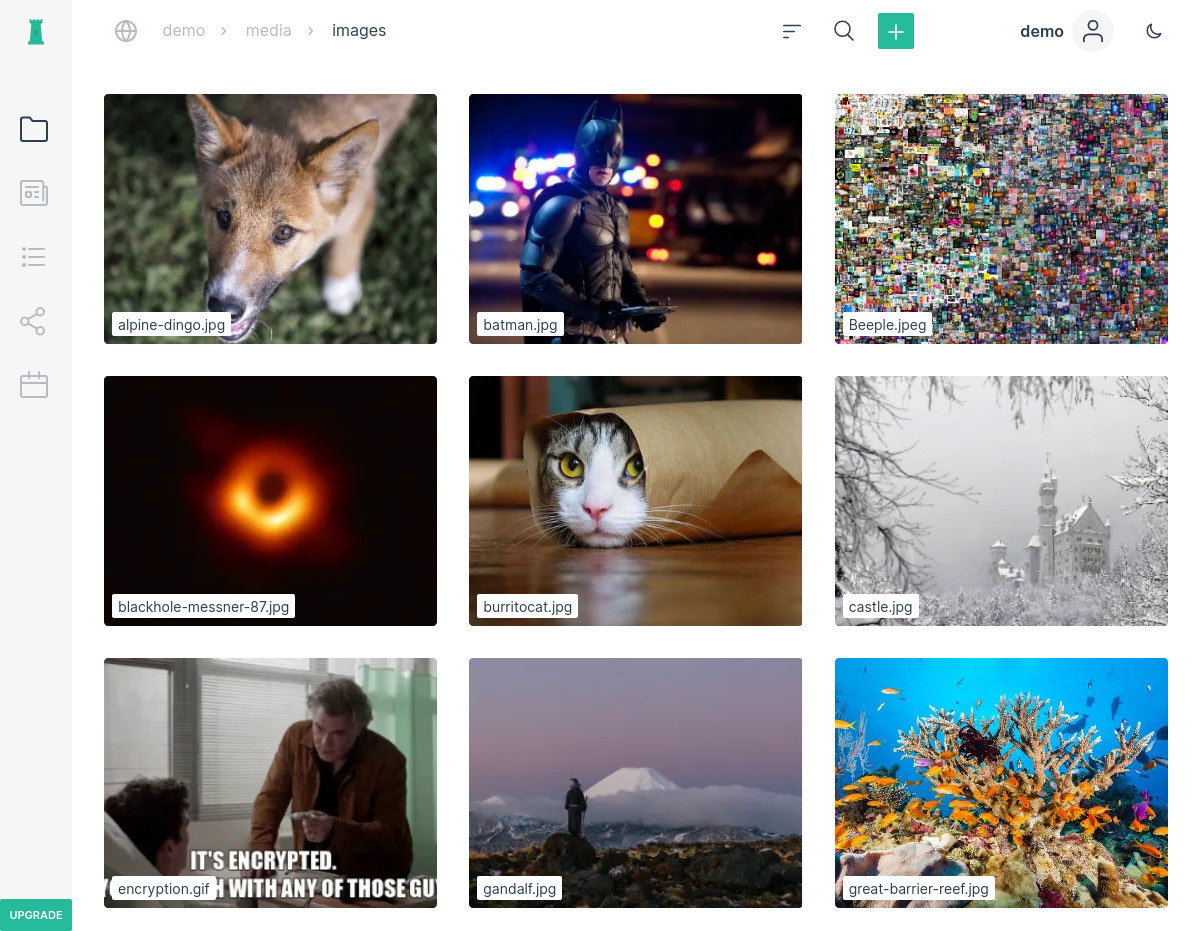
\includegraphics[width=0.8\linewidth]{images/peergos.jpg}
    \caption{Plataforma web de Peergos}
    \label{fig:peergos}
\end{figure}

Otro aspecto de gran interés es el sistema registro de usuarios. Las claves públicas y los nombres de usuario se almacenan en una estructura de datos global de solo adición,
con los  nombres asignados por orden de llegada. Esto requiere consenso para garantizar la singularidad de los nombres de usuario.
Aquí es también donde se almacena el ID del nodo IPFS del servidor (o servidores) responsables de sincronizar las escrituras del
usuario. El problema de la implementación realizada por Peergos es que se necesita de uno o varios servidores centralizado
que denominan \textit{Corenode} que mantienen y sirven este registro para los usuarios.

Este registro es en sí la base de datos de usuarios, la autenticación se maneja mediante un sistema de clave pública-privada
guardada en el navegador del usuario. Se usa una contraseña definida por el usuario para el acceso a la cuenta.

Peergos es una plataforma muy completa y que ofrece una gran cantidad de funcionalidades que escapan del alcance de este proyecto.
Se puede considerar esta plataforma como referencia del potencial de IPFS, y aunque no es perfecta y tiene sus limitaciones, es un buen ejemplo de lo que se puede lograr con esta tecnología.

\section{Filecoin}

Filecoin\cite{filecoinDecentralizedStorageNetwork} es una plataforma de almacenamiento descentralizado en la nube basada en
blockchain. La plataforma utiliza su propia criptomoneda,llamada Filecoin (FIL), para facilitar e incentivar las transacciones dentro
de la red.

Filecoin no está dirigido a consumidores (usuarios de a pie) ya que realmente es un mercado para proveedores de almacenamiento en la nube. Puede llegar
a ser de interés para el futuro de este proyecto ya que se podría integrar el sistema con Filecoin para ofrecer un servicio parecido
a un proveedor de almacenamiento en la nube, pero con distintos proveedores que compiten entre sí para ofrecer el mejor servicio.

\section{Sailplane}\label{sec:sailplane}

Sailplane se describe como una plataforma para \textit{'Compartir archivos de forma colaborativa punto a punto en el navegador'}.

Sailplane, al igual que este proyecto, usa OrbitDB como el componente central de sus sistema\footnote{Este proyecto fue descubierto
    hacia el final del desarrollo de este trabajo de fin de grado por lo que este hecho es más bien una casualidad.}.
Como ya se ha explicado previamente, OrbitDB es una base de datos distribuida. Sailplane implementa un backend de almacenamiento
conocido como un \textit{store}. Un store en OrbitDB se refiere a una instancia de una base de datos individual que se sincroniza
automáticamente con otros stores del mismo tipo mediante la red IPFS.

Sailplane ha implementado su propio store llamado \textit{orbit-db-fsstore}\cite{TabcatOrbitdbfsstoreCustom}. Este representa
un sistema de ficheros montado sobre OrbitDB que se puede sincronizar con otras instancias de la base de datos, lo que permite
mantener y compartir un sistema de ficheros sincronizado entre varios usuarios. Este sistema de archivos se puede encriptar aunque no es necesario.

\begin{figure}[H]
    \centering
    \small
    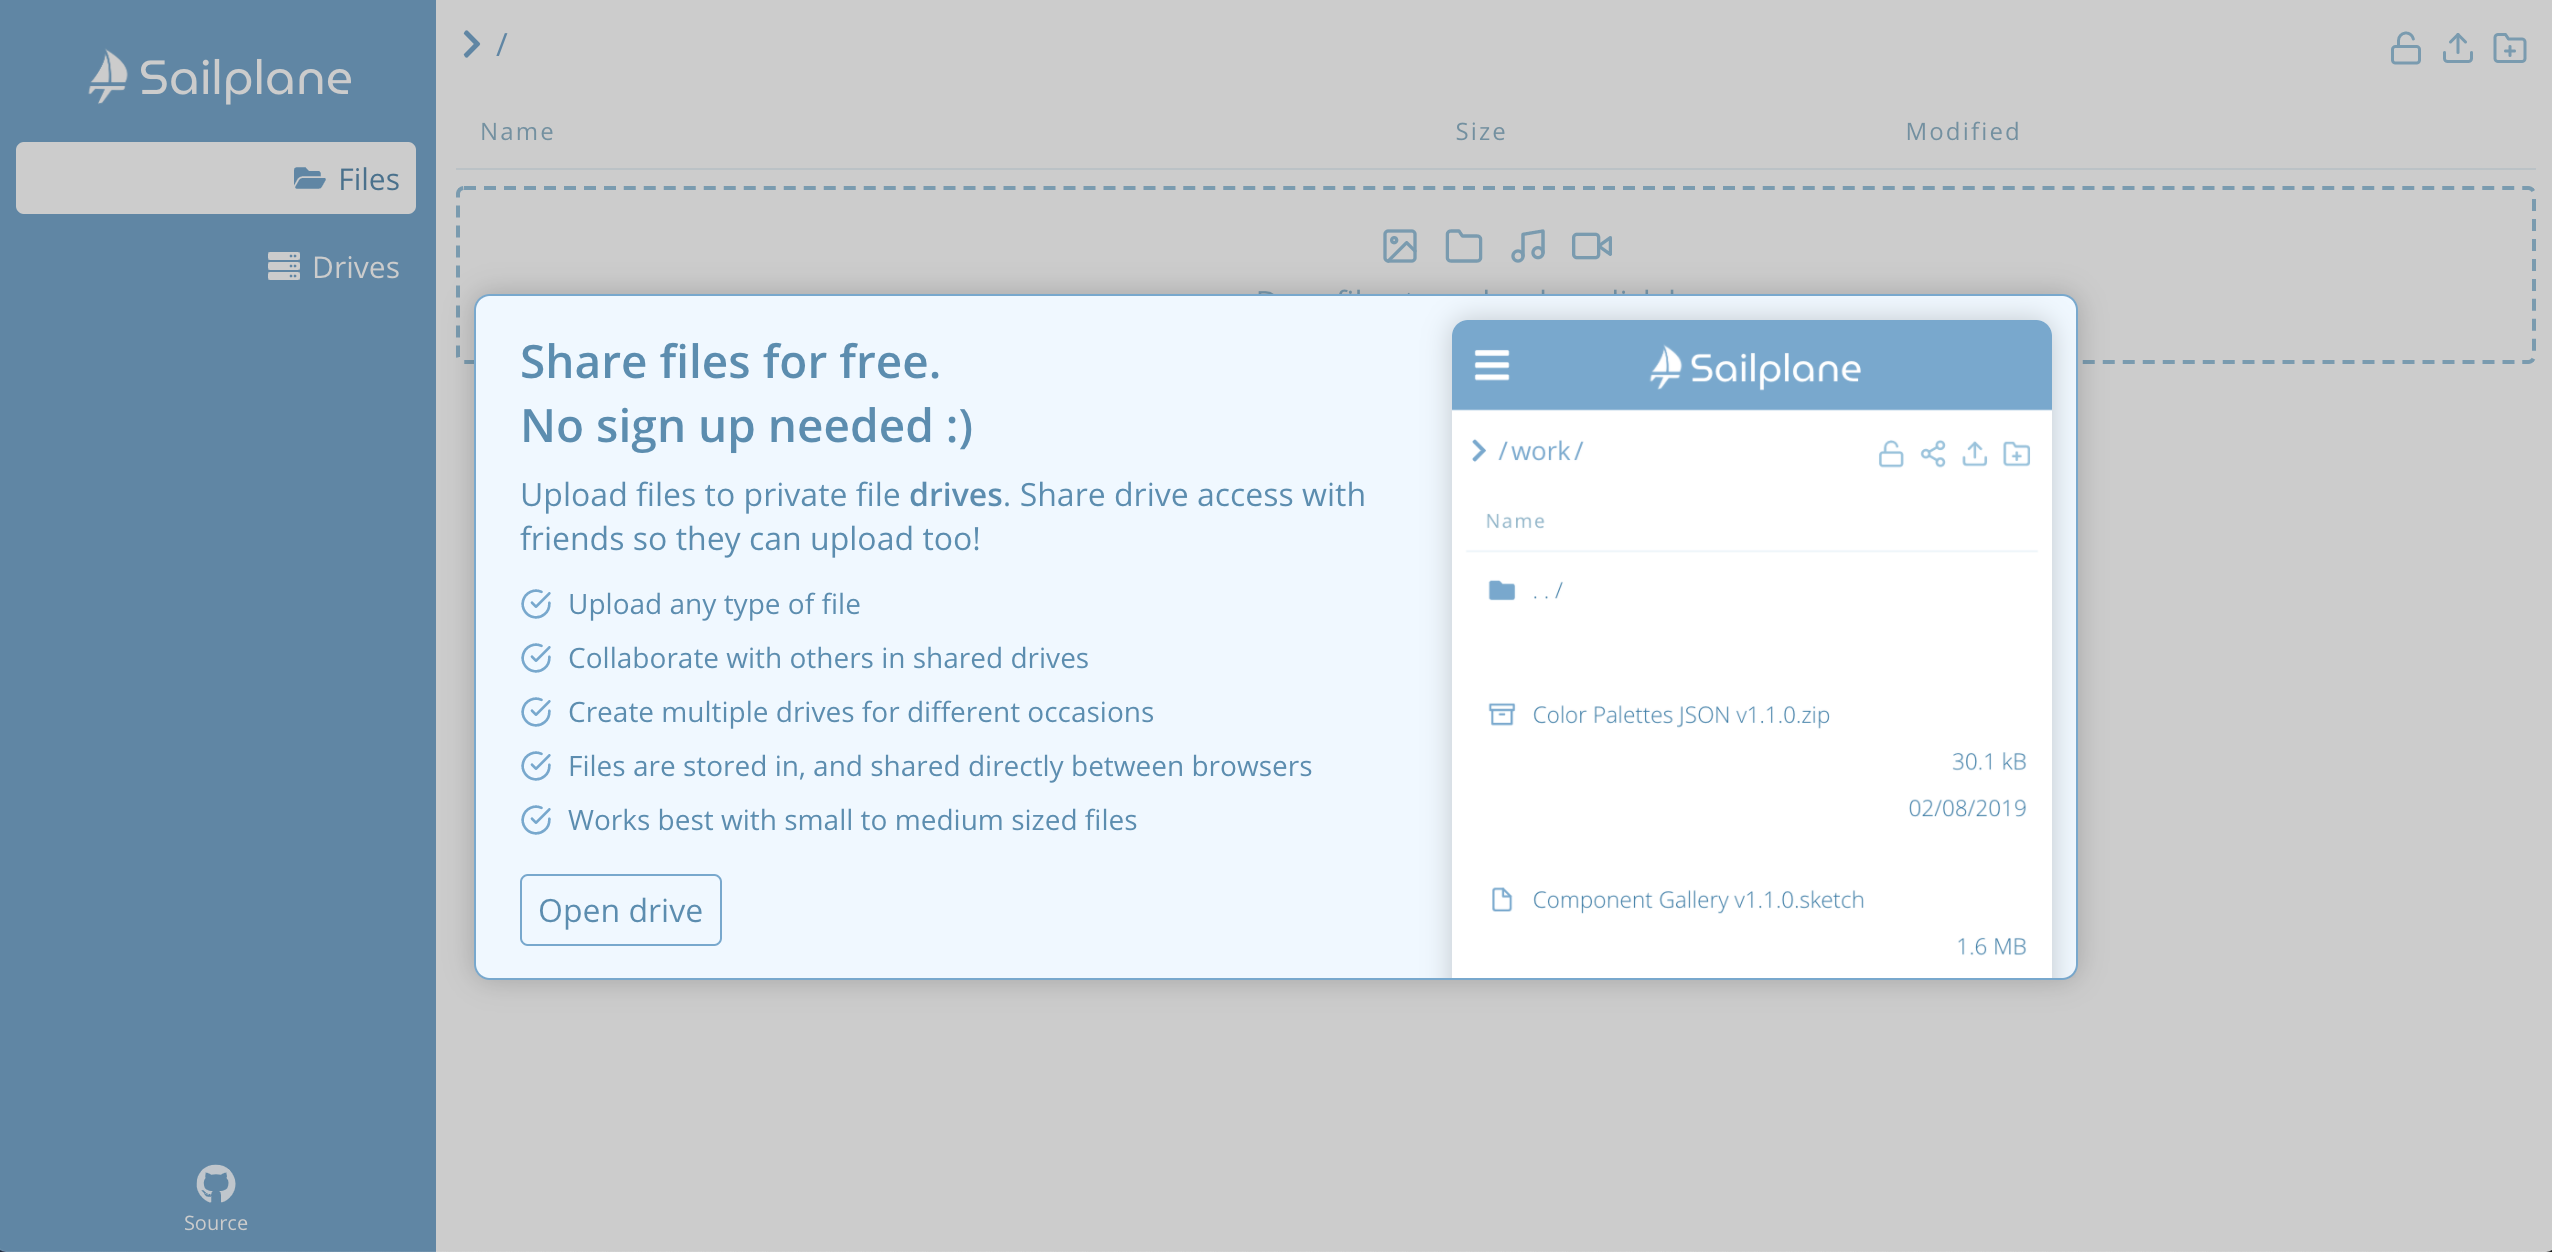
\includegraphics[width=\linewidth]{images/sailplane.png}
    \caption{Aplicación web de Sailplane}
    \label{fig:sailplaneweb}
\end{figure}

Sailplane ofrece una implementación de un nodo IPFS personalizado llamado
\\\textit{sailplane-node}\cite{Sailplanenode2023}, que expone una interfaz para interactuar directamente con el store.
Existe también una web que hace uso de este nodo y ofrece:
\begin{itemize}
    \item Un sistema de ficheros en el navegador basado en \textit{drives} (discos virtuales) compartidos.
    \item Un sistema de registro automático y autocontenido. Esto sirve para que la hora de compartir un drive este pueda
          ver los usuarios con los que puede compartirlo.
\end{itemize}

\begin{figure}[H]
    \centering
    \small
    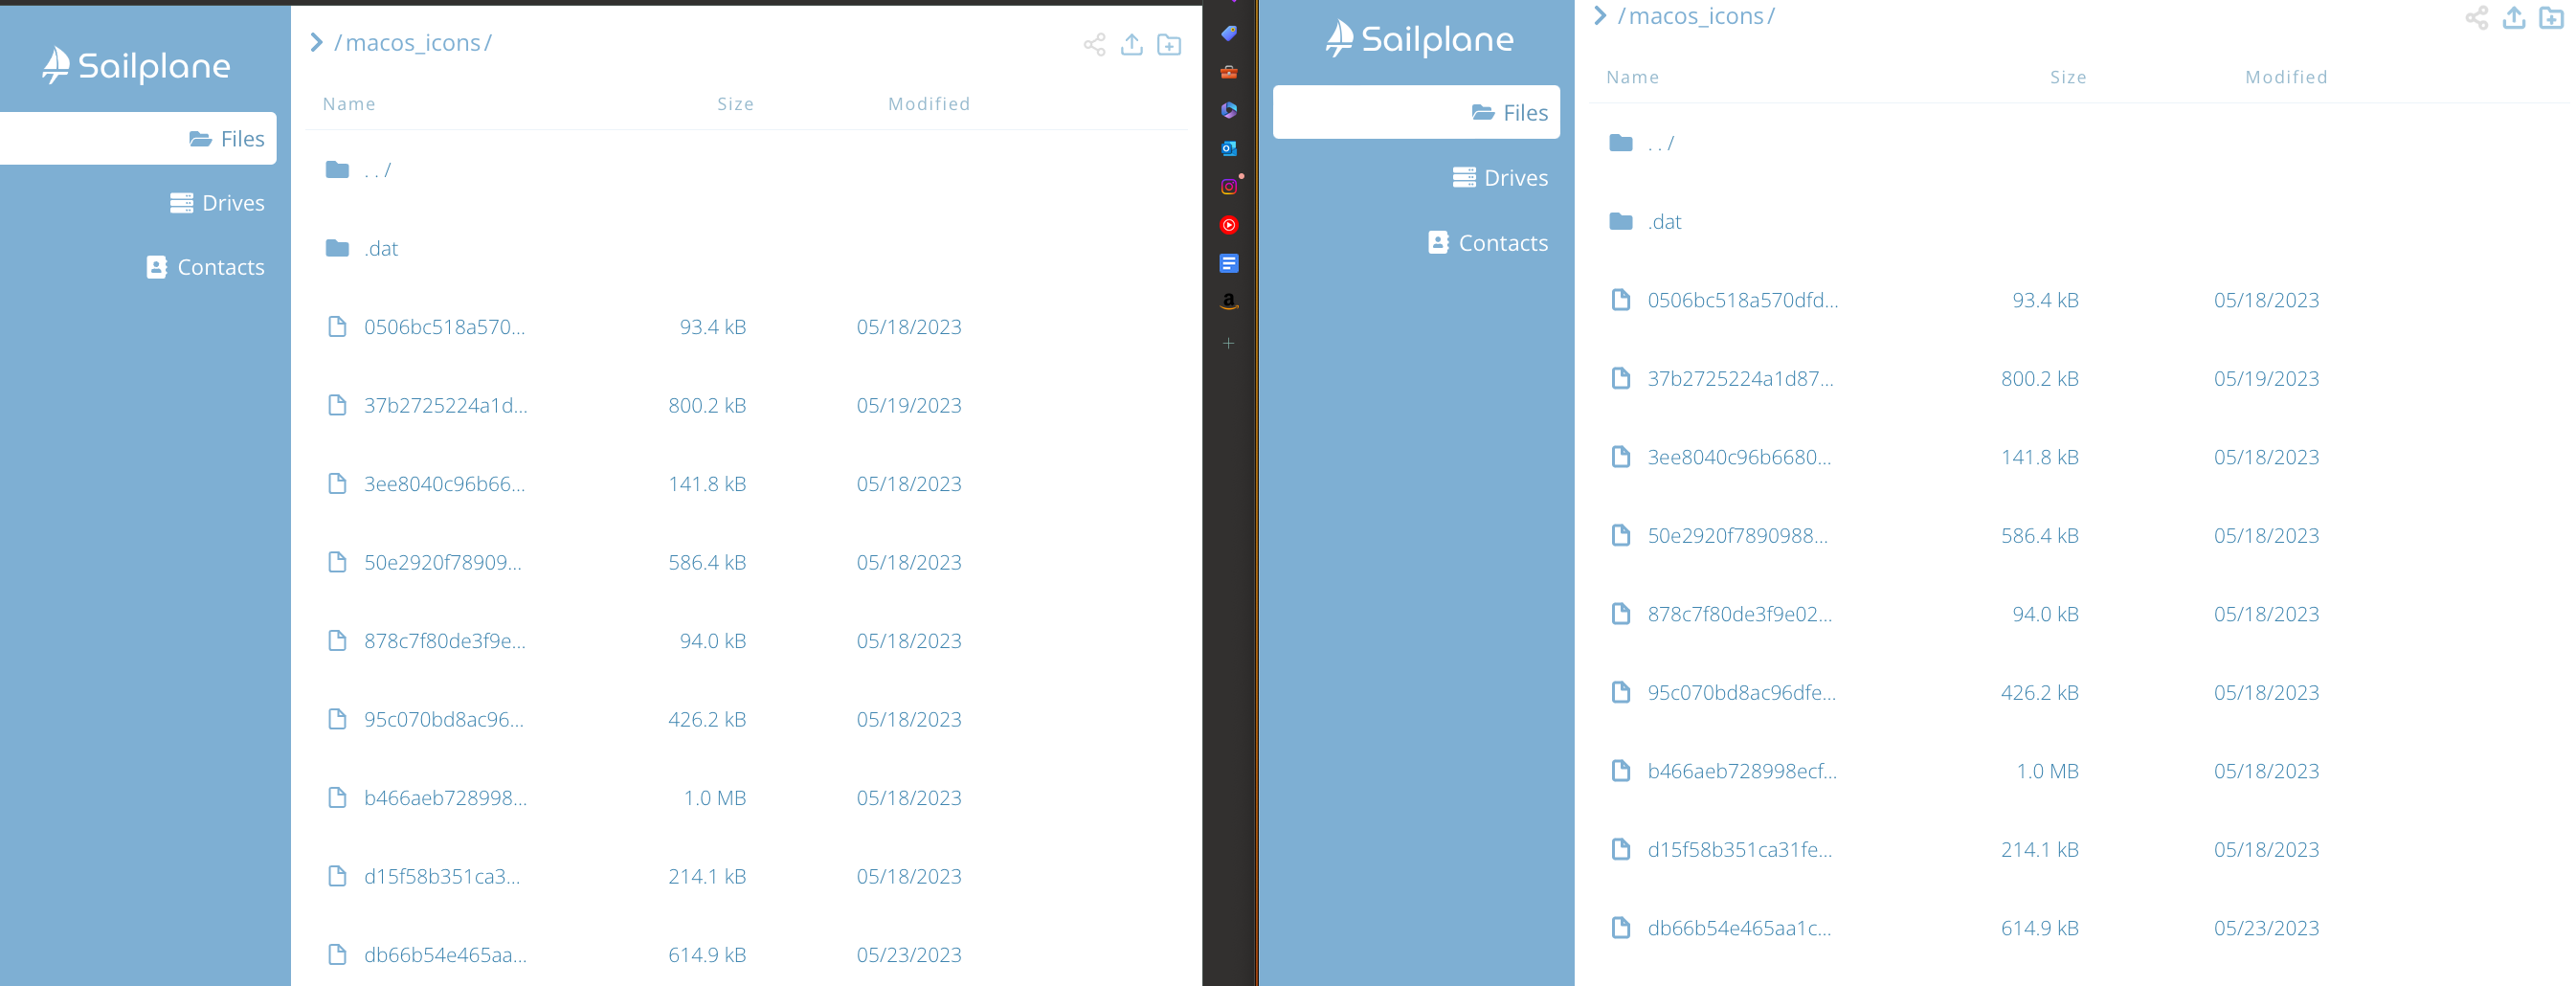
\includegraphics[width=\linewidth]{images/saiplanesynced.png}
    \caption{Dos nodos Sailplane sincronizando el el mismo drive}
    \label{fig:sailplanewebsync}
\end{figure}

Lo que más destaca de Sailplane es  la implementación de un sistema de ficheros montado sobre OrbitDB.
Esto es algo que se explorará más adelante en la el capítulo \ref{chap:7trabajosfuturos}: '\nameref{chap:7trabajosfuturos}'.
El uso de OrbitDB para un sistema de registro automático y autocontenido es algo que también se ha implementado en la propuesta, aunque como se ha
comentado previamente, el descubrimiento de este proyecto ocurrió ya habiendo desarrollado esta característica.

\section{Fileverse}
Fileverse es una plataforma de almacenamiento que se integra con IPFS y que permite guardar, compartir y acceder a archivos desde cualquier dispositivo.


Actualmente ofrece dos productos, ambos en formato de aplicación web:
\begin{itemize}
    \item Fileverse Solo: Una aplicación web para subir y compartir archivos sin autenticación. El usuario sube un archivo y recibe un enlace que puede compartir con otros usuarios. En la figura \ref{fig:fileverse} se puede observar un ejemplo de uso.
    \item Fileverse Portals: Una aplicación web que integra autenticación basada en blockchain. Es un espacio de trabajo para la gestión de archivos sobre blochain (e IPFS) y la creación de contenido. Está en fase de pruebas y no se puede acceder.
\end{itemize}
\begin{figure}[H]
    \centering
    \small
    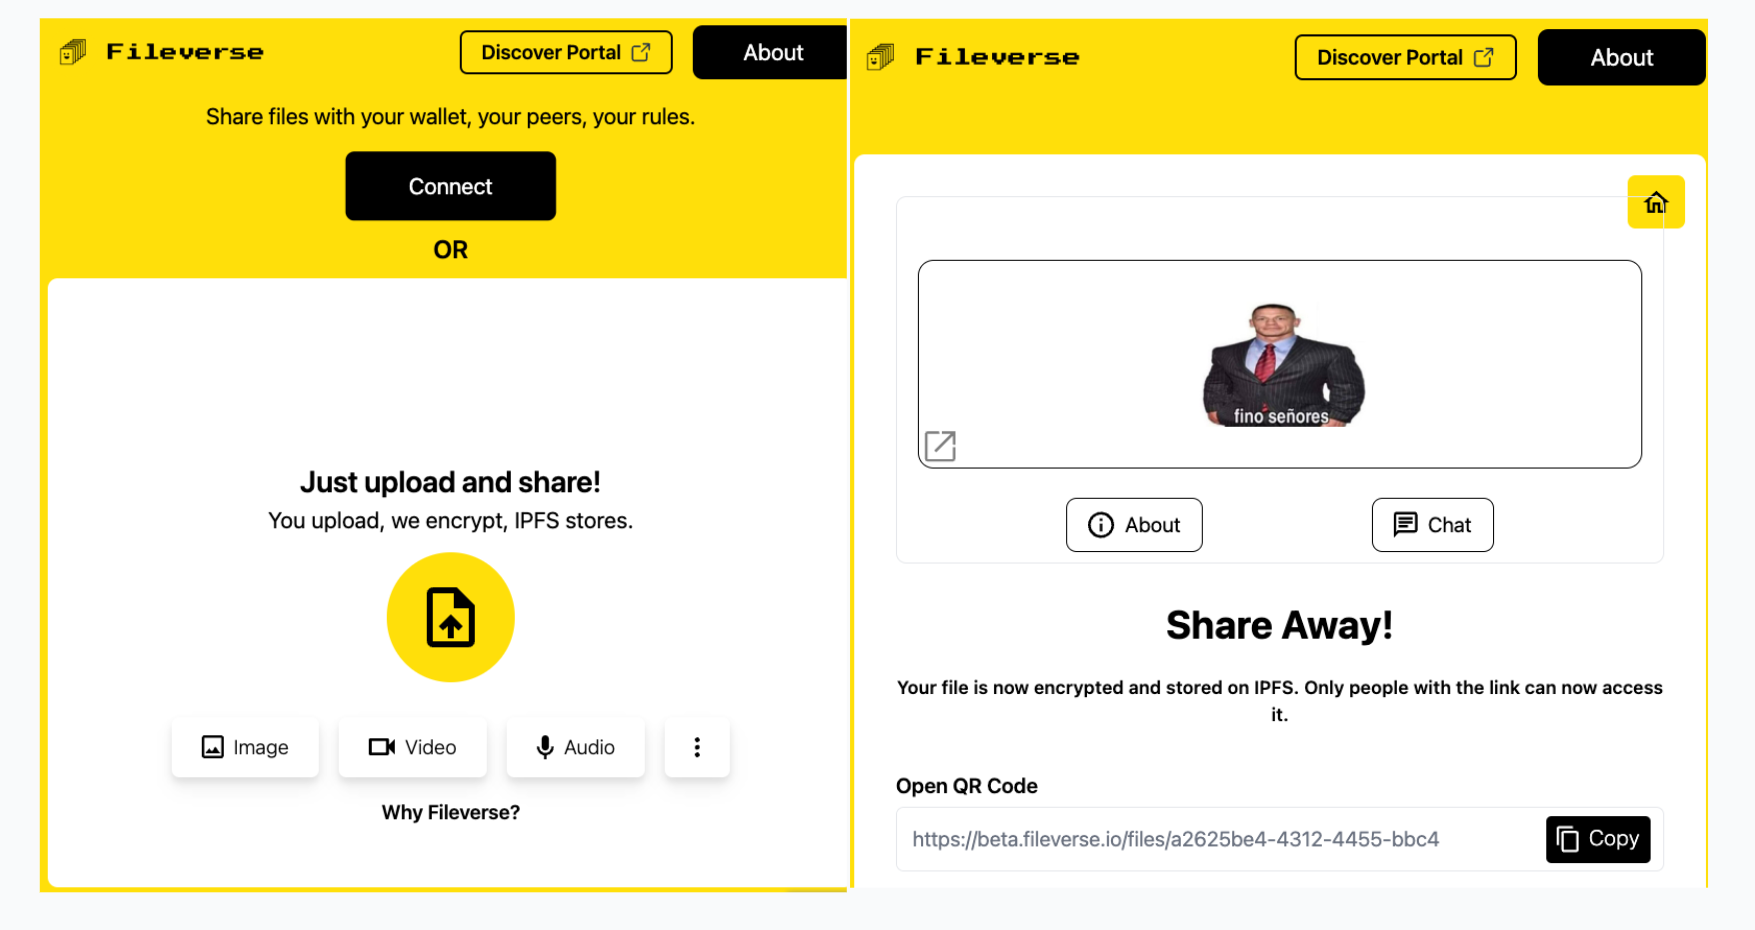
\includegraphics[width=\linewidth]{images/fileverse.png}
    \caption{Aplicación web de Fileverse para subir archivos}
    \label{fig:fileverse}
\end{figure}

El servicio que ofrece Fileverse Solo es muy simple: el usuario sube un archivo y recibe un enlace que puede pasar a otras personas para descargar dicho archivo.
Esta caso de uso es muy similar al que se propone en este proyecto, aunque con algunas diferencias. El uso de una
aplicación web resulta más sencillo que una línea de comandos, pero no integra cuentas de usuario ni formas de acceder o gestionar comparticiones pasadas.


\section{Conclusión}

Como se puede observar en este capítulo existen varias implementaciones de sistemas de almacenamiento y compartición de
archivos basadas en IPFS. Como opinión personal, ninguna presenta un servicio comparable al de los grandes
proveedores centralizados de almacenamiento en la nube. Tanto en términos de facilidad de uso, como de funcionalidades y
fiabilidad.

Esto se debe a que detrás de estos servicios hay una gran infraestructura e inversión que no es comparable a estos proyectos
que tienen un carácter más experimental, investigativo y proviene de equipos de desarrollo mucho más limitados. Aún así, estos proyectos son un buen ejemplo de lo que se puede lograr con IPFS y
han sido de gran ayuda a la hora de realizar este proyecto, en particular Sailplane y Peergos.


\chapter{Desarrollo de IPFShare}\label{chap:4desarrollo}
Se ha denominado IPFShare al sistema de intercambio de archivos desarrollado en este proyecto.
\section{Requisitos y definición del sistema}
En esta sección se definen los requisitos funcionales y no funcionales que debe integrar el sistema propuesto.
\subsection{Requisitos funcionales}
\begin{itemize}[noitemsep,after=\vspace{-0.6\baselineskip}]
  \item Un usuario debe poder autenticarse en el sistema.
  \item Un usuario debe poder compartir archivos y directorios con uno o varios usuarios.
  \item Un usuario debe poder descargar archivos y directorios compartidos por otros usuarios del sistema.
  \item A la hora de compartir un archivo un usuario debe poder elegir con qué otros usuarios del sistema compartirlo.
  \item Un usuario debe tener posibilidad de hacer grupos de compartición.
  \item Cuando un usuario comparta recursos con otros usuarios, estos deben recibir una notificación.
  \item Un usuario debe poder interactuar las comparticiones que ha realizado.
  \item Un usuario debe poder interactuar las comparticiones que le han realizado.
\end{itemize}
\subsection{Requisitos no funcionales}
\begin{itemize}[noitemsep,after=\vspace{-0.4\baselineskip}]
  \item El sistema debe proporcionar una interfaz de usuario intuitiva y fácil de usar.
  \item El sistema debe implementar servicios de seguridad en torno a la autenticación.
  \item El sistema debe proporcionar medidas de seguridad para los archivos compartidos.
  \item El sistema debe proporcionar un servicio o mecanismos de identificación de usuario portable.
  \item Las transacciones y eventos del sistema deben ser relativamente instantáneos.
\end{itemize}
Hay que destacar que este sistema no propone la sincronización de archivos que normalmente se asocia con los sistemas de
almacenamiento en la nube. Incluir el desarrollo de esta funcionalidad en el sistema propuesto no es algo trivial.
La sincronización de datos en tiempo real es un tópico muy complejo y se sale
del alcance de este proyecto. Sin embargo, en la sección de \nameref{chap:7trabajosfuturos} dentro de las posibles
mejoras se propone una posible implementación de esta funcionalidad.
\section{Arquitectura y diseño}

Uno de los objetivos de este trabajo es comparar la viabilidad de IPFS como alternativa a los sistemas centralizados.
En esta sección se presenta una arquitectura simplificada para un sistema de intercambio de archivos centralizado habitual.
Después se contrastará con la alternativa descentralizada propuesta.

\subsection{Arquitectura de un sistema de intercambio de archivos centralizado habitual}

Como se puede observar en la figura \ref{fig:centralizedarch}, la arquitectura de un sistema de intercambio de archivos
requiere de varios puntos de acceso centralizados para funcionar\footnote{Este diseño se ha ideado tomando como referencia los siguientes recursos:
  \cite{chakrabortySystemDesignAnalysis2020} y
  \cite{systemdesignSystemDesignInterview2023}.}.En un caso real esta arquitectura podría ser más compleja, pero para este
ejemplo se ha simplificado para centrarse en los puntos clave.

Existe una clara separación conceptual de las distintos componentes, aunque pueden estar ubicados en
el mismo servidor físico, en varios, o incluso, cada servicio en varios servidores físicos. Esto depende de la escala
del sistema y de las necesidades de rendimiento y disponibilidad.

\begin{itemize}[noitemsep,after=\vspace{-0.4\baselineskip}]
  \item \textbf{Almacenamiento cloud:} el almacén donde se guardarán los chunks de ficheros proporcionados por el servicio
        de procesamiento de ficheros, Amazon S3 es un ejemplo de un servicio de estas característica.
        \item\textbf{Servicio de procesamiento de ficheros:} es el encargado atender y llevar a cabo las peticiones de usuario relacionadas con ficheros.
  \item \textbf{Servicio de autenticación:} gestiona la autenticación de los usuarios. Contiene los datos de los usuarios y sus credenciales.
  \item \textbf{Servicio de metadatos:} se encarga de enviar las notificaciones de los usuarios. Cuando un cliente
        comparte un fichero con otro, el cliente envía también una serie de metadatos sobre esta acción que acaba de realizar.
        Estos metadatos se pueden usar para gran variedad de propósitos. En este caso se usan para implementar un servicio de notificaciones basado en colas de mensajes.
\end{itemize}
\afterpage{
  \begin{sidewaysfigure}
    \centering
    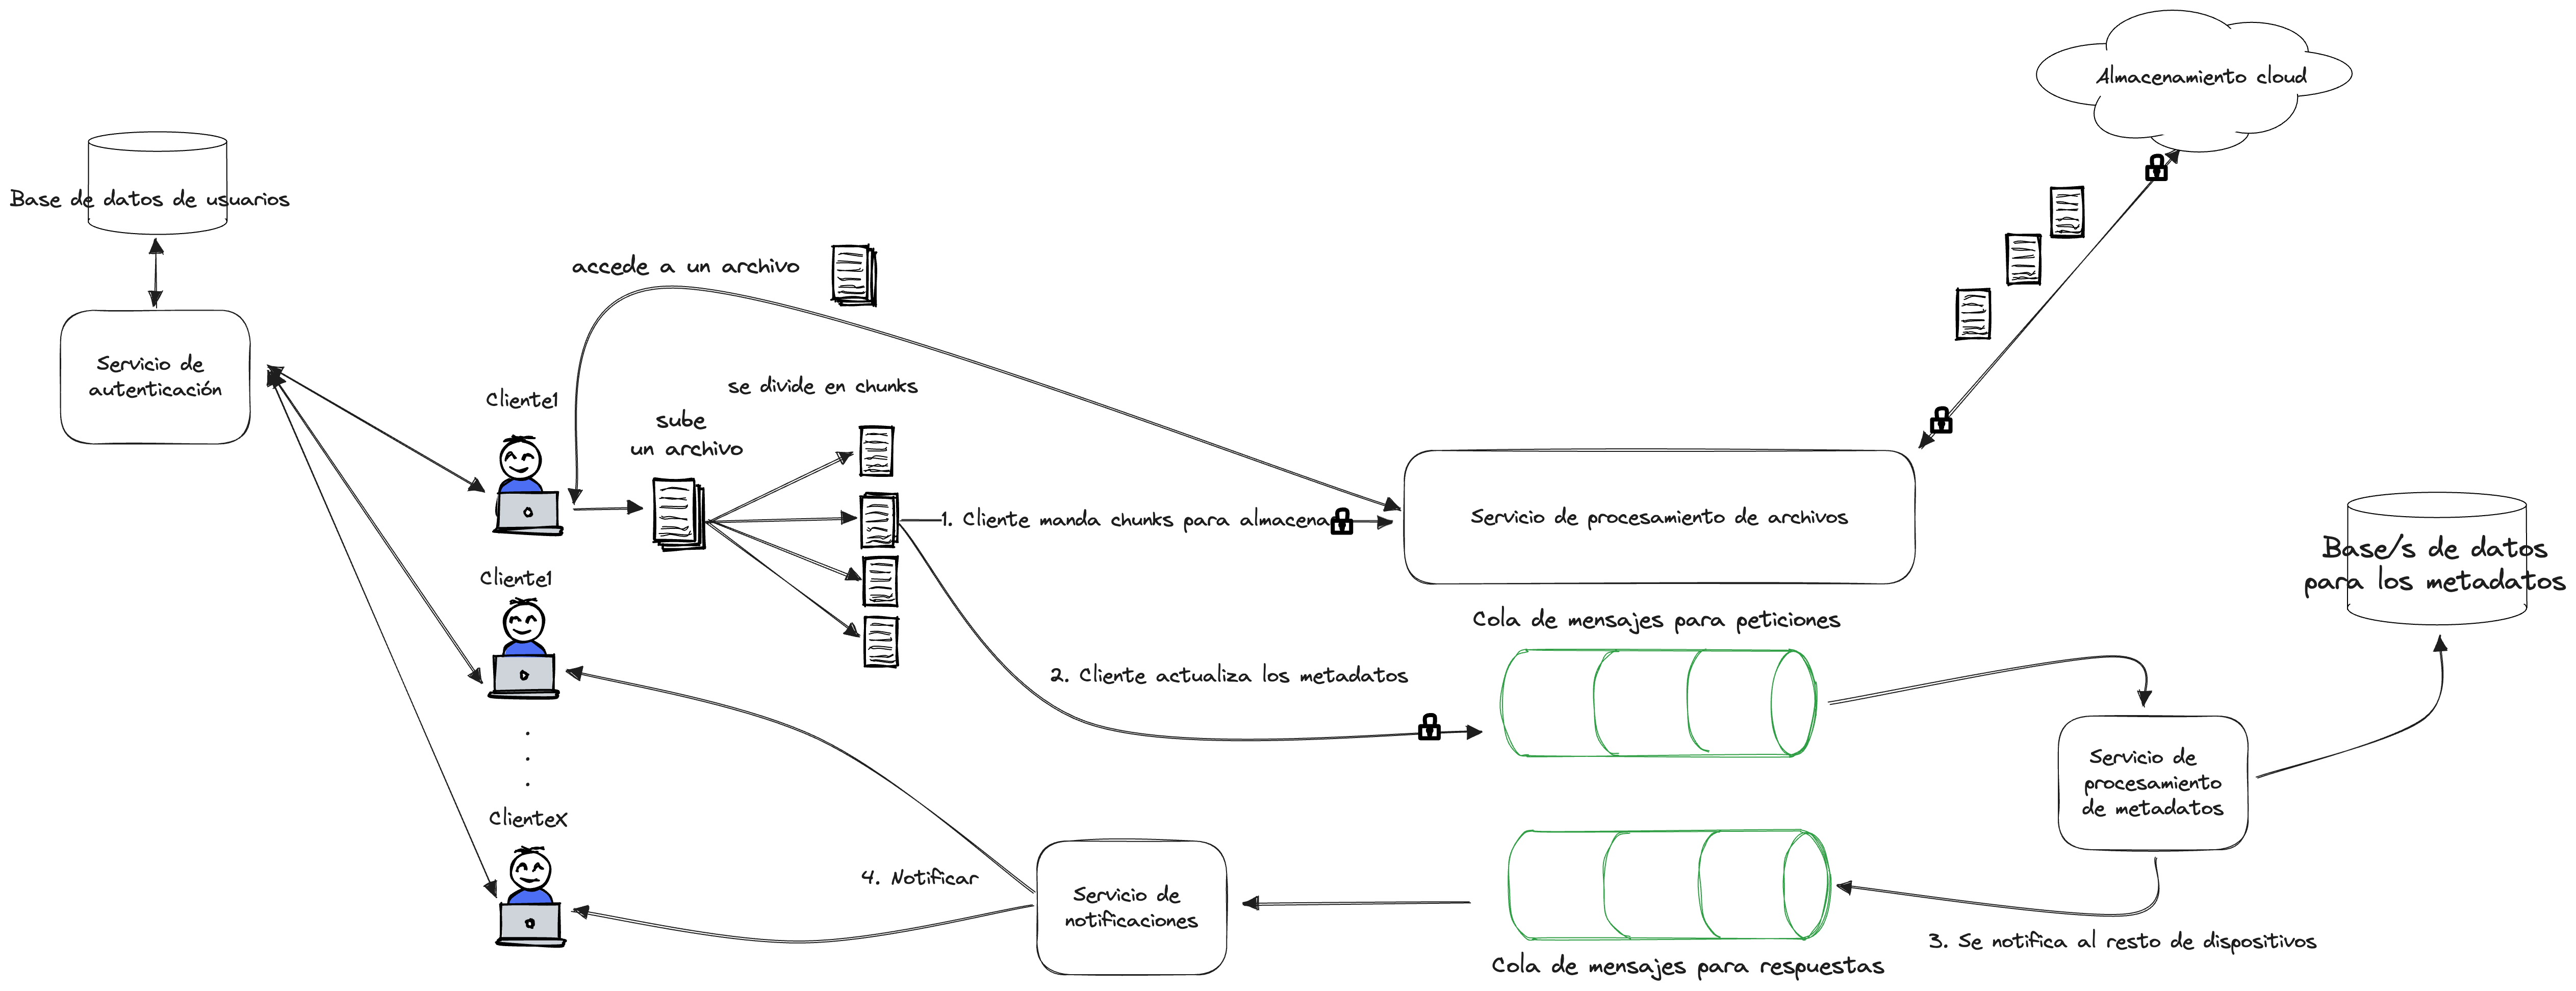
\includegraphics[width=\textwidth]{images/diagramacentral.png}
    \caption{Posible arquitectura de un servicio centralizado de archivos}
    \label{fig:centralizedarch}
  \end{sidewaysfigure}
}

Cuando un cliente quiere compartir un fichero, este divide el archivo en trozos más pequeños llamados chunks\footnote{En un servicio de compartición de archivos, los archivos se subdividen en fragmentos o chunks para mejorar la eficiencia de la transferencia de datos, permitiendo la transmisión paralela y la reanudación de las transferencias interrumpidas, así como facilitar la distribución del almacenamiento y reducir la redundancia de datos.}.
Envía a través de una conexión segura (socket tpc sobre TLS por ejemplo) estos chunks que componen el archivo al servicio de procesamiento de ficheros.
Este servicio se encarga de guardar los chunks en el almacenamiento cloud y de mandar los metadatos a la cola de mensajes.
El servicio de metadatos procesa de forma asíncrona estos metadatos, extrayendo la información pertinente que identifique
a los usuarios y el recurso compartido. Después envía una notificación a los usuarios que corresponda.

Dado que el servicio de autenticación posee datos de los usuarios, cuando un usuario quiera enviar un archivo puede
pedir esta al servicio de autenticación, el incluso se podría combinar con el servicio de metadatos para brindar otras funcionalidades como ver los recursos que se le han compartido o los usuarios con los que se ha compartido.

Bajo este sistema los clientes deben saber de antemano dónde se ubican estos servicios para poder interactuar con
ellos. Estos servicios podrían ser provistos por entidades externas, por lo que el sistema no sería completamente autocontenido, existiendo dependencias en sistemas centralizados de terceros.

\subsection{Arquitectura de IPFShare: un sistema de intercambio de archivos descentralizado}
En comparacion con la arquitectura anterior (figura \ref{fig:centralizedarch}), la arquitectura de IPFShare (figura \ref{fig:ipfssharearch}) es completamente descentralizada.
\section{Tecnologías}
\subsection{Tecnologías propuestas}
\subsection{Tecnologías usadas}


\section{Implementación}


\begin{minted}{typescript}
import OrbitDB from "orbit-db"
// eslint-disable-next-line @typescript-eslint/ban-ts-comment
// @ts-ignore
import AccessController from "orbit-db-access-controllers/interface"
import DocumentStore from "orbit-db-docstore"
import { IdentityProvider } from "orbit-db-identity-provider"

export interface RegistryEntry {
    peerId: string
    orbitdbIdentity: string // DID
    username: string // alias
  }

export abstract class Registry<S, DocType> {
    abstract accessController: AccessController
    abstract store: S
    abstract open(): Promise<void>
    abstract create(): Promise<void>
    abstract replicate(): Promise<void>
    abstract close(): Promise<void>
    abstract addUser(user: DocType): Promise<void>
    abstract getUser(entryId: string): Promise<DocType | undefined>
    abstract updateUser(entryId: string, updates: Partial<DocType>): Promise<void>
    abstract searchUsers(queryFn: (entry: DocType) => boolean): Promise<DocType[]>
    abstract deleteUser(entryId: string): Promise<void>
  }
\end{minted}

\input{secciones/05_Evaluación.tex}

\chapter{Resultados y conclusiones}\label{chap:6resultados}

Con esta implementación se han cumplido practicamente la totalidad de los objetivos del proyecto enumerados en la sección \ref{sec:objetivos}: \nameref{sec:objetivos}. Se ha desarrollado un sistema de intercambio de ficheros basado en IPFS, mediante una aplicación de escritorio. Este sistema permite a los usuarios compartir archivos de forma segura y confiable, sin necesidad de ningún proveedor central de ningún tipo. Integra capacidades de encriptación y control de acceso para garantizar la seguridad de los archivos compartidos. La integración de cuentas de usuario, aunque sin la posibilidad de hacer grupos. También se puede elegir contactos con los que compartir. Por último se integra un sistema de notificaciones para el que
los usuarios puedan recibir avisos de nuevos archivos compartidos, o de cambios en los archivos compartidos.

El objetivo de investigar sobre IPFS y su funcionamiento para entender cómo funciona el protocolo y cómo se puede utilizar para el sistema propuesto también se ha cumplido. Se ha realizado un estudio con una profundidad adecuada al ámbito y alcance de este proyecto. Se han explicado conceptos de IPFS, su funcionamiento, arquitectura, algoritmo de intercambio de bloques, identificación basada en contenido, hasta su estructura de datos.
Con estos conceptos como base se ha profundizado en el ecosistema en torno a IPFS, con objetivo de comprender la madurez y viabilidad de esta tecnología, así como de las herramientas basadas en esta que se pueden utilizar para el sistema propuesto. Sobre esto último:

Tras el satisfactorio resultado obtenido se podría pensar que IPFS y su ecosistema están lo suficientemente avanzados como para ser utilizados en un sistema de producción. Sin embargo, tras el desarrollo de este proyecto se ha podido comprobar que aún están en una fase temprana de su evolución. Esto se debe a que se han encontrado varios problemas durante el desarrollo del proyecto, algunos de ellos se han podido solucionar, pero otros no. Estos problemas se han debido principalmente a la falta de documentación y a la inmadurez o falta de mantenimiento de algunas herramientas.

Uno de los grandes obstáculos en el entorno de NodeJS para IPFS es la falta de soporte y mantenimiento de los paquetes de tipos de Typescript.
Ciertos paquetes como \textit{orbitdb-identity-provider} tienen sus paquetes de tipos desactualizados, están erróneamente implementados o la documentación está obsoleta. Para solventar estos problemas se ha tenido que recurrir al uso de \textit{//@ts-ignore} en múltiples ocasiones, esta
es una directiva que indica al compilador de Typescript que haga caso omiso a los errores de tipos que se producen en la línea siguiente. Este tipo de directivas está
generalmente desaconsejado y hace que el uso de Typescript pierda sentido al desarrollar, ya que no realizan las comprobaciones de tipado.

Para el paquete de \textit{orbitdb-identity-provider} se ha tenido que recurrir a hacer \textit{fork} del repositorio para poder arreglar
dos errores para el proveedor de identificación basado en DIDs, que es el usado por IPFShare.

Esta falta o mala documentación también se traslada a las propias implementaciones de IPFS. Un ejemplo de esto es la difusa relación entre UnixFS y el MFS, tal como se presenta en la documentación. Esta no esclarece bien las diferencias entre ambos, ni como se relacionan entre sí. Aunque se pueden encontrar explicaciones en los foros oficiales
por parte de los desarrolladores\cite{ItPossibleShare}, no es una solución satisfactoria para un desarrollador que se enfrenta a estas tecnologías por primera vez.
\\Otro ejemplo son las diferencias que existen entre las implementaciones de IPFS, no funcionan exactamente igual ni dan el mismo soporte de tecnologías. Existen también pocos recursos online tanto para usuarios como desarrolladores, lo que dificulta la adopción de IPFS.
\\Esta clase de situaciones hace hace que sea difícil para los desarrolladores aprovechar el potencial de IPFS como un sistema de archivos distribuido y mutable. Este proyecto podría haberse implementado en Go, pero JavaScript y el entorno de NodeJS son tremendamente más populares entre desarrolladores 67.9\% de profesionales saben JS respecto un 11.83\% Go\footnote{Fuente: \cite{StackOverflowDeveloper}}.

Como conclusión final: IPFS se considera una tecnología innovadora con el potencial de transformar la forma en que los archivos se almacenan y comparten en internet. Si bien no es adecuada para todos los casos de uso, es una opción valiosa para aquellos que buscan alternativas descentralizadas en el almacenamiento y distribución de archivos. Aunque presenta algunas limitaciones, como preocupaciones de privacidad y posibles desafíos de escalabilidad, la comunidad de desarrollo continúa trabajando en mejoras para superar estas limitaciones y fortalecer la eficiencia y confiabilidad de IPFS. Este trabajo es una muestra del potencial de esta tecnología, y de su aparente sinfín de aplicaciones que ofrece gracias a su naturaleza distribuida, el uso de árboles de Merkle y la inmutabilidad de datos que estos proveen.

\chapter{Trabajos futuros}\label{chap:7trabajosfuturos}

En este capítulo se exploran las posibles vías de expansión y mejoras para el proyecto en el futuro.

\section{Mejoras en la interfaz de usuario}
La línea de comandos como interfaz de IPFShare es adecuada para un prototipo, aunque esto no se traslada a un
producto final que busque ser usado por usuarios no técnicos. Por tanto, una mejora obvia sería la implementación de una interfaz gráfica de usuario.

Esta interfaz gráfica se podría proveer mediante una aplicación web o de escritorio. En ambos casos se podría aprovechar la implementación actual de IPFShare, ya que
esta se ha desarrollado en NodeJS, lo que permite que se pueda ejecutar en el navegador o en el escritorio mediante Electron\cite{BuildCrossplatformDesktop}.

Esta mejora no es trivial, ya que el soporte de OrbitDB en el navegador requiere de servidores WebRTCStar \cite{OrbitDBrtc2023} para el correcto descubrimiento de nodos en la red. Esto es algo que se podría solucionar con la implementación de un servidor propio, esto implicaría añadir un componente centralizado que
haría que el sistema no fuera completamente autocontenido y distribuido.

\section{Uso de streams para el consumo de contenido en memoria}
Dentro de la implementación actual se han integrado dos comandos que exploran este concepto. Estos son \texttt{ipfshare cat} y \texttt{ipfshare ls}.
Estos comandos permiten consumir contenido de IPFS en memoria mediante streams, lo que habilita el uso de estos comandos en scripts y otras herramientas.

El uso de concepto en otros comandos merece la pena ser explorado por las ventajas de consumo de disco y memoria que ofrece.

\section{Mejoras en el sistema de notificaciones}
En la implementación actual las notificaciones son creadas por los propios usuarios para sí mismos al llegar nuevas entradas
del ShareLog dirigidas a estos. En ciertas ocasiones el evento sobre el que se realizan estas acciones no se dispara, por lo que
las notificaciones pueden pasar desapercibidas. La solución a este problema consiste en el uso de bases de datos locales
en las que se añaden las comparticiones que se tienen del ShareLog, y se comprueba si ya se han mostrado previamente.

El algoritmo de comprobación de duplicados que implementa esta funcionalidad:
\begin{minted}{typescript}

async ensureLocalUpToDate() { 
    await this.localSharedWithMeStore.load()
    await this.localSharedWithOthersStore.load()
    await this.store.load()
    const localSharedWithMeEntries = this.localSharedWithMeStore.iterator().collect()
    const localSharedWithOtherEntries = this.localSharedWithOthersStore.iterator().collect()
    this.store.iterator().collect().forEach(
        (entry) => { 
            (async () => {
                if (entry.payload.value.senderId === this._orbitdb.id &&
                    localSharedWithOtherEntries.filter(async (localEntry) => {
                        return localEntry.payload.value.shareCID.toString() === entry.payload.value.shareCID.toString()
                    }).length == 0) {
                    await this.localSharedWithOthersStore.add(entry.payload.value)
                }
                if (entry.payload.value.recipients.includes(this._orbitdb.id)
                    &&
                    entry.payload.value.senderId !== this._orbitdb.id
                    &&
                    localSharedWithMeEntries.filter(
                        (localEntry) => localEntry.payload.value.shareCID.toString() === entry.payload.value.shareCID.toString()
                    ).length === 0
                ) {
                    await this.localSharedWithMeStore.add(entry.payload.value)
                    const value: ShareLogEntry = entry.payload.value
                    logger.info('New share available, ${JSON.stringify(value)}')
                    notify(value)
                }
            })()
        })
}
\end{minted}

Como se puede observar este método tiene una complejidad temporal de $O(n^2)$. Esto se debe a que en el peor de los casos, para cada entrada en \texttt
{this.store} (n entradas), se ejecuta una operación de filtrado tanto en \texttt{localSharedWithOtherEntries} como en
\\\texttt{localSharedWithMeEntries} (en el peor de los casos, cada operación de filtrado puede recorrer todos los elementos, que son de tamaño n). Por
lo tanto, la complejidad total es proporcional al cuadrado del número de elementos, es decir, $O(n^2)$. No es una implementación eficiente, pero es la única que se ha encontrado que funciona correctamente, es por ello que se incluye en esta sección.


\section{Mejoras en el sistema de encriptación}

El algoritmo de encriptación que IPFShare utiliza es AES-256-CBC, que es seguro y comúnmente usado. Sin embargo, no es la mejor opción para su uso específico en IPFShare. AES-256-CBC es un algoritmo de cifrado en bloque que no puede paralelizarse, como resultado, el cifrado de archivos grandes puede resultar lento.


\section{Integración de un sistema de ficheros en tiempo real sobre OrbitDB}
Como ya se comentó en el la sección \ref{sec:sailplane}, Sailplane ha implementado un sistema de ficheros montado sobre OrbitDB. Esto es algo que se podría implementar en IPFShare ampliando enormemente las capacidades y casos de uso que IPFShare cubre actualmente.

Se podría ampliar la implementación del store de Sailplane para que este soporte la encriptación de los archivos, y así poder ofrecer un sistema de ficheros encriptado capaz de sincronizarse en tiempo real y automáticamente entre los usuarios que tengan la instancia del store.

\section{Integración de un sistema de ficheros en tiempo real sobre IPFS}

En la anterior sección se ha discutido la posibilidad de usar OrbitDB como la base sobre la que montar un sistema de ficheros en tiempo real.
Sin embargo, también se podría implementar un sistema de ficheros en tiempo real sobre IPFS. Actualmente existen esta funcionalidad en IPFS
mediante el uso del MFS, pero no incorpora ningún tipo de encriptación ni sistema de control de acceso.

Se podría manipular el MFS manualmente para recrear sus funcionalidades pero añadiendo una capa de encriptación por la que pasarían los archivos antes de ser añadidos al MFS. A la hora de la consumición de estos archivos se deberían desencriptar antes de ser consumidos.


\chapter*{Anexo}


\begingroup
\renewcommand*{\arraystretch}{1.5}
\small % reducir tamaño de fuente
\begin{longtable}{|>{\raggedright\arraybackslash}m{2.4cm}|>{\raggedright\arraybackslash}m{2.8cm}|>{\raggedright\arraybackslash}m{2.8cm}|>{\raggedright\arraybackslash}m{2.8cm}|>{\raggedright\arraybackslash}m{2.8cm}|}
    \hline
    \textbf{Característica} & \textbf{IP/TCP}                                                                                                                                                                        & \textbf{OSI}                                                                                                                                                                                                                                         & \textbf{X.25}                                                                                                                                                                                                                                                                                                                                                                    & \textbf{SNA}                                                                                                                                                                                                                                                                           \\ \hline
    Modelo                  & Suite de protocolos                                                                                                                                                                    & Modelo de referencia                                                                                                                                                                                                                                 & Protocolo de enlace                                                                                                                                                                                                                                                                                                                                                              & Suite de protocolos                                                                                                                                                                                                                                                                    \\ \hline
    Capas                   & 4 (TCP/IP)                                                                                                                                                                             & 7                                                                                                                                                                                                                                                    & 3                                                                                                                                                                                                                                                                                                                                                                                & 7                                                                                                                                                                                                                                                                                      \\ \hline
    Año de lanzamiento      & 1974 (TCP) / 1981 (IP)                                                                                                                                                                 & 1984                                                                                                                                                                                                                                                 & 1976                                                                                                                                                                                                                                                                                                                                                                             & 1974                                                                                                                                                                                                                                                                                   \\ \hline
    Enfoque                 & Conmutación de paquetes                                                                                                                                                                & Conmutación de paquetes y circuitos                                                                                                                                                                                                                  & Conmutación de circuitos                                                                                                                                                                                                                                                                                                                                                         & Conmutación de paquetes y circuitos                                                                                                                                                                                                                                                    \\ \hline
    Estándar                & IETF                                                                                                                                                                                   & ISO                                                                                                                                                                                                                                                  & CCITT (ahora ITU-T)                                                                                                                                                                                                                                                                                                                                                              & IBM                                                                                                                                                                                                                                                                                    \\ \hline
    Orientación             & Red global                                                                                                                                                                             & Interoperabilidad                                                                                                                                                                                                                                    & Redes de área amplia (WAN)                                                                                                                                                                                                                                                                                                                                                       & Redes empresariales                                                                                                                                                                                                                                                                    \\ \hline
    Funcionalidades         & Transmisión de datos, enrutamiento, control de flujo, control de congestión, conexión y desconexión                                                                                    & Transmisión de datos, enrutamiento, control de flujo, control de congestión, conexión y desconexión, servicios de presentación y aplicación                                                                                                          & Transmisión de datos, control de flujo, conexión y desconexión                                                                                                                                                                                                                                                                                                                   & Transmisión de datos, enrutamiento, control de flujo, control de congestión, conexión y desconexión, servicios de presentación y aplicación                                                                                                                                            \\ \hline
    Uso en los años 90      & Muy popular, base del Internet                                                                                                                                                         & Intento de reemplazar a TCP/IP, pero fracasó en la adopción generalizada                                                                                                                                                                             & Utilizado en redes de área amplia (WAN), especialmente en Europa                                                                                                                                                                                                                                                                                                                 & Utilizado en redes empresariales, especialmente en sistemas mainframe de IBM                                                                                                                                                                                                           \\ \hline
    Descripción             & Un modelo que se basa en la suite de protocolos TCP/IP para transmitir datos por Internet. El modelo es más simple y flexible que el modelo OSI y se usa ampliamente en la actualidad. & Un modelo que se basa en la suite de protocolos OSI para estandarizar la comunicación entre sistemas abiertos. El modelo segmenta múltiples funciones que el modelo IPTCP agrupa en capas únicas y define los servicios e interfaces para cada capa. & Un modelo que se basa en la suite de protocolos X.25 para proporcionar una conexión virtual entre terminales y computadoras a través de una red pública de conmutación de paquetes. El modelo fue uno de los primeros en ofrecer una comunicación confiable entre dispositivos remotos, pero ha sido reemplazado por tecnologías más rápidas y eficientes como Frame Relay e IP. & Un modelo que se basa en la suite de protocolos SNA para integrar los recursos informáticos distribuidos en una red jerárquica. El modelo fue desarrollado por IBM para conectar sus sistemas mainframe y periféricos, pero ha perdido popularidad frente a los modelos basados en IP. \\ \hline
    \caption[Comparación de IP/TCP, OSI, X.25 y SNA en los años 90]{Comparación de IP/TCP, OSI, X.25 y SNA en los años 90. Fuentes: \cite{dasTCPIPProtocol2022}, \cite{ProtocoloControlTransmision2023}, \cite{ProtocolWars2023}, \cite{TCPIPModela} \cite{cooneySNAOSIVs2007a} \cite{LayersOSIModel2017a}}
    \label{tab:comparacion-protocolos-90}
\end{longtable}
\endgroup









\bibliographystyle{IEEEtran}
\bibliography{ref.bib}

\addcontentsline{toc}{chapter}{Bibliografía}
%%-----------------------------------------------
%% Anexos
\appendix
\clearpage
\addcontentsline{toc}{chapter}{Anexo}
\chapter*{Anexo}


\begingroup
\renewcommand*{\arraystretch}{1.5}
\small % reducir tamaño de fuente
\begin{longtable}{|>{\raggedright\arraybackslash}m{2.4cm}|>{\raggedright\arraybackslash}m{2.8cm}|>{\raggedright\arraybackslash}m{2.8cm}|>{\raggedright\arraybackslash}m{2.8cm}|>{\raggedright\arraybackslash}m{2.8cm}|}
    \hline
    \textbf{Característica} & \textbf{IP/TCP}                                                                                                                                                                        & \textbf{OSI}                                                                                                                                                                                                                                         & \textbf{X.25}                                                                                                                                                                                                                                                                                                                                                                    & \textbf{SNA}                                                                                                                                                                                                                                                                           \\ \hline
    Modelo                  & Suite de protocolos                                                                                                                                                                    & Modelo de referencia                                                                                                                                                                                                                                 & Protocolo de enlace                                                                                                                                                                                                                                                                                                                                                              & Suite de protocolos                                                                                                                                                                                                                                                                    \\ \hline
    Capas                   & 4 (TCP/IP)                                                                                                                                                                             & 7                                                                                                                                                                                                                                                    & 3                                                                                                                                                                                                                                                                                                                                                                                & 7                                                                                                                                                                                                                                                                                      \\ \hline
    Año de lanzamiento      & 1974 (TCP) / 1981 (IP)                                                                                                                                                                 & 1984                                                                                                                                                                                                                                                 & 1976                                                                                                                                                                                                                                                                                                                                                                             & 1974                                                                                                                                                                                                                                                                                   \\ \hline
    Enfoque                 & Conmutación de paquetes                                                                                                                                                                & Conmutación de paquetes y circuitos                                                                                                                                                                                                                  & Conmutación de circuitos                                                                                                                                                                                                                                                                                                                                                         & Conmutación de paquetes y circuitos                                                                                                                                                                                                                                                    \\ \hline
    Estándar                & IETF                                                                                                                                                                                   & ISO                                                                                                                                                                                                                                                  & CCITT (ahora ITU-T)                                                                                                                                                                                                                                                                                                                                                              & IBM                                                                                                                                                                                                                                                                                    \\ \hline
    Orientación             & Red global                                                                                                                                                                             & Interoperabilidad                                                                                                                                                                                                                                    & Redes de área amplia (WAN)                                                                                                                                                                                                                                                                                                                                                       & Redes empresariales                                                                                                                                                                                                                                                                    \\ \hline
    Funcionalidades         & Transmisión de datos, enrutamiento, control de flujo, control de congestión, conexión y desconexión                                                                                    & Transmisión de datos, enrutamiento, control de flujo, control de congestión, conexión y desconexión, servicios de presentación y aplicación                                                                                                          & Transmisión de datos, control de flujo, conexión y desconexión                                                                                                                                                                                                                                                                                                                   & Transmisión de datos, enrutamiento, control de flujo, control de congestión, conexión y desconexión, servicios de presentación y aplicación                                                                                                                                            \\ \hline
    Uso en los años 90      & Muy popular, base del Internet                                                                                                                                                         & Intento de reemplazar a TCP/IP, pero fracasó en la adopción generalizada                                                                                                                                                                             & Utilizado en redes de área amplia (WAN), especialmente en Europa                                                                                                                                                                                                                                                                                                                 & Utilizado en redes empresariales, especialmente en sistemas mainframe de IBM                                                                                                                                                                                                           \\ \hline
    Descripción             & Un modelo que se basa en la suite de protocolos TCP/IP para transmitir datos por Internet. El modelo es más simple y flexible que el modelo OSI y se usa ampliamente en la actualidad. & Un modelo que se basa en la suite de protocolos OSI para estandarizar la comunicación entre sistemas abiertos. El modelo segmenta múltiples funciones que el modelo IPTCP agrupa en capas únicas y define los servicios e interfaces para cada capa. & Un modelo que se basa en la suite de protocolos X.25 para proporcionar una conexión virtual entre terminales y computadoras a través de una red pública de conmutación de paquetes. El modelo fue uno de los primeros en ofrecer una comunicación confiable entre dispositivos remotos, pero ha sido reemplazado por tecnologías más rápidas y eficientes como Frame Relay e IP. & Un modelo que se basa en la suite de protocolos SNA para integrar los recursos informáticos distribuidos en una red jerárquica. El modelo fue desarrollado por IBM para conectar sus sistemas mainframe y periféricos, pero ha perdido popularidad frente a los modelos basados en IP. \\ \hline
    \caption[Comparación de IP/TCP, OSI, X.25 y SNA en los años 90]{Comparación de IP/TCP, OSI, X.25 y SNA en los años 90. Fuentes: \cite{dasTCPIPProtocol2022}, \cite{ProtocoloControlTransmision2023}, \cite{ProtocolWars2023}, \cite{TCPIPModela} \cite{cooneySNAOSIVs2007a} \cite{LayersOSIModel2017a}}
    \label{tab:comparacion-protocolos-90}
\end{longtable}
\endgroup








%%---------------------------------------------------------
\end{document}
